% File clic2021.tex
% May 2021

%% Based on the style files for CLiC-IT-2019, which were, in turn,
%% Based on the style files for CLiC-IT-2014, which were, in turn,
%% Based on the style files for ACL-2014, which were, in turn,
%% Based on the style files for ACL-2013, which were, in turn,
%% Based on the style files for ACL-2012, which were, in turn,
%% based on the style files for ACL-2011, which were, in turn, 
%% based on the style files for ACL-2010, which were, in turn, 
%% based on the style files for ACL-IJCNLP-2009, which were, in turn,
%% based on the style files for EACL-2009 and IJCNLP-2008...
%% Based on the style files for EACL 2006 by 
%% e.agirre@ehu.es or Sergi.Balari@uab.es
%% and that of ACL 08 by Joakim Nivre and Noah Smith

\documentclass[11pt]{article}
\usepackage[a4paper]{geometry} 
\usepackage{clic2023} % imports CLiC-it 2023 layout style
\usepackage{times} % font 
\usepackage{xurl} % splits URL in multiple lines
\usepackage[italian,english]{babel}
\usepackage{latexsym} 
\pagenumbering{gobble} % does not display page numbering
\usepackage{xcolor}
\usepackage{multirow}
\usepackage{todonotes}
\usepackage{subcaption}
\usepackage{amssymb}
\usepackage{float}
\usepackage{cuted}
\usepackage{soul}
\usepackage{xcolor}

\definecolor{lightgreen}{RGB}{0, 180, 0}
\definecolor{lightred}{RGB}{214, 0, 0}

\newcommand{\hlg}[1]{{\sethlcolor{lightgreen}\hl{#1}}}
\newcommand{\hlr}[1]{{\sethlcolor{lightred}\hl{#1}}}


\newcommand{\bs}[0]{$\blacksquare$}

\newcommand{\Ni}{({\em i})~}
\newcommand{\Nii}{({\em ii})~}
\newcommand{\Niii}{({\em iii})~}

\newcommand{\abc}[1]{{\color{blue} #1}}
\newcommand{\paolo}[1]{{\color{red} #1}}

\newcommand{\todoA}[1]{\todo[color=blue!40]{A: #1}}
\newcommand{\todoP}[1]{\todo[color=red]{P: #1}}

\newcommand{\itodo}[1]{\todo[inline]{#1}}

\newcommand{\dsENcorpus}{IFU-22-EN}
\newcommand{\dsITcorpus}{IFU-22-IT}
\newcommand{\dsENclassification}{IFS-EN}
\newcommand{\dsITclassification}{IFS-IT}
\newcommand{\dsENforecasting}{IFSS-EN-223K}
\newcommand{\dsITforecasting}{IFSS-IT-30K}

\newcommand{\mbert}{\mbox{mBERT$_{base}$}}
\newcommand{\imbert}{\mbox{Incel mBERT}}
\newcommand{\umbert}{\mbox{UmBERTo}}
\newcommand{\albert}{\mbox{AlBERTo}}
\newcommand{\iumbert}{\mbox{Incel UmBERTo}}
\newcommand{\ialbert}{\mbox{Incel AlBERTo}}

\newcommand{\hsdfb}{\mbox{HSD-FB}}
\newcommand{\hsdtw}{\mbox{HSD-TW}}
\newcommand{\ami}{\mbox{AMI-20}}


\newcommand{\dsENclassificationtrain}{IFS-EN$_{\mbox{tr}}$} % Incel Forum Supervised, English, 5203 instances
\newcommand{\dsENclassificationdev}{IFS-EN$_{\mbox{de}}$} % Incel Forum Supervised, English, 5203 instances
\newcommand{\dsENclassificationtest}{IFS-EN$_{\mbox{te}}$} % Incel Forum Supervised, English, 5203 instances

\newcommand{\enforum}{\textit{Incels.is}}
\newcommand{\itforum}{\textit{Il forum dei brutti}}


%\setlength\titlebox{5cm}

% You can expand the titlebox if you need extra space
% to show all the authors. Please do not make the titlebox
% smaller than 5cm (the original size); we will check this
% in the camera-ready version and ask you to change it back.


  \title{Hate Speech Detection in Italian Incel Forums \\ Using Bilingual Data for Pre-Training and Fine-Tuning}

\author{\textbf{Paolo Gajo, Alberto Barrón Cedeño, Silvia Bernardini, Adriano Ferraresi} \\
  University of Bologna, Italy \\
  {\tt paolo.gajo@studio.unibo.it}\\
  {\tt \{a.barron, silvia.bernardini, adriano.ferraresi\}@unibo.it}}

\date{}

\begin{document}
\maketitle
\begin{abstract}
\textbf{English.}~In this paper we approach the problem of improving the performance of hate speech detection models in
% cross-lingual and cross-domain settings, in
an Italian forum frequented by incels.
% , short for ``involuntary celibates''
We pre-train monolingual (Italian) and multilingual Transformer models on corpora built from two incel forums, one in Italian and one in English, using masked language modeling. Then, we fine-tune the models on combinations of English and Italian datasets binary-annotated for hate speech.
% , built from incel forums and mainstream social media sites.
% with binary labels which indicate whether a post contains hate speech or not. The Italian training datasets are compiled from mainstream social media (Twitter and Facebook), while the English dataset is built by gathering posts from the English incel forum. The models' performance is evaluated on the Italian incel forum dataset.
Testing them on a hate speech dataset obtained from the Italian incel forum shows that the best results are achieved by training multilingual models on bilingual training data,
rather than using monolingual models on Italian-only data, emphasizing the importance of in-domain data, even when training and target languages differ.

% HS identification in cross-lingual and cross-domain settings. We do so by employing Transformer models, pre-trained on monolingual (Italian) and bilingual (Italian-English) corpora. We fine-tune these models on various combinations of English- and Italian-language datasets, all annotated for HS. The English-language dataset pertains to the so-called community of ``incels'', short for ``involuntary celibates'', while the ones in Italian are compiled from mainstream social media sites (Twitter and Facebook). We then evaluate the performance of the models on an Italian-language dataset built from the contents of an Italian incel forum. Our experiments with model domain adaptation via training on the masked language modeling task and fine-tuning on different combinations of datasets show that the best results are obtained not by training solely using Italian data, but with a combination of Italian and English data. This shows the importance of using in-domain data for training, even when training and test data are in different languages.

\end{abstract}

\begin{abstract-alt}
\textrm{\bf{Italiano.}}~In questo studio affrontiamo il problema di migliorare le prestazioni di modelli per l'identificazione di discorsi di odio in un forum italiano di incel.
%  , abbreviazione di ``celibi involontari''.
Addestriamo modelli Transformer monolingue (italiano) e multilingue su corpora ottenuti da due forum di incel, uno in italiano e uno in inglese, con il masked language modeling. Quindi, facciamo il fine-tuning dei modelli su dataset in italiano e inglese con annotazioni binarie indicanti se un post esprime odio.
%  , costruiti a partire da social media di vasto utilizzo e forum di incel.
Valutandoli su un dataset ottenuto da un forum italiano di incel, osserviamo che i risultati migliori si ottengono addestrando modelli multilingue su combinazioni bilingue di dataset, sottolineando l'importanza di utilizzare dati appartenenti allo stesso contesto linguistico, anche con lingue differenti di addestramento e valutazione.
 
%  . A questo scopo, impieghiamo modelli Transformer, pre-addestrati su corpora monolingui (italiano) e bilingui (italiano-inglese). Abbiamo effettuato il fine-tuning di questi modelli su varie combinazioni di dataset in lingua inglese e italiana, tutti annotati per i discorsi d'odio. Il dataset inglese riguarda la comunità dei c.d. ``incel'', abbreviazione inglese di ``celibi involontari'', mentre quelli italiani sono costruiti partendo da social media di vasto utilizzo (Twitter e Facebook). Valutiamo le prestazioni dei modelli su un dataset in lingua italiana costruito a partire dai contenuti di un forum italiano di incel. Gli esperimenti di adattamento dei modelli a questo contesto linguistico attraverso l'addestramento sulla task del masked language modeling e il fine-tuning su diverse combinazioni di dataset dimostrano che i risultati migliori si ottengono non solo con l'addestramento su dati in italiano, ma con una combinazione di dati in italiano e in inglese. Questo dimostra l'importanza di utilizzare dati provenienti dallo stesso contesto linguistico per l'addestramento, anche quando i dati di addestramento e di test sono in lingue diverse.
\end{abstract-alt}


\section{Introduction}

Hate speech, broadly defined as language that expresses hatred towards a targeted group or is intended to be derogatory, humiliating, or insulting to the members of the group~\cite{davidson-2017-automated-hate}, has become an increasingly prevalent and dangerous phenomenon in the past years \cite{matamoros-fernandezRacismHateSpeech2021}.
% The rapid rise of social media platforms has enabled the dissemination of hateful and offensive rhetoric, with tangible negative consequences, such as increased prejudice towards minority groups and the escalation of hate crimes \cite{peliconInvestigatingCrosslingualTraining2021}.
 A specific area of concern in the realm of hate speech is the online spaces known as the ``Manosphere'', where misogynous discourse in particular has become increasingly rampant~\cite{ribeiro2021evolution-manosphere}.
% These spaces are characterized by the adoption of the ``Red Pill'' philosophy, which promotes a toxic idea of masculinity and traditional gender roles, and has been linked to the rise in misogynous and racist discourse~\cite{gingAlphasBetasIncels2019-manosphere}.
Specifically, the incel (short for ``involuntary celibate'') community within the Manosphere has been identified as one that frequently engages in hateful, misogynous, and racist speech~\cite{nagle-2017-kill-normies,jakiOnlineHatredWomen2019}.
% Given the gravity of the phenomenon, especially in these environments, the development of effective hate speech detection systems is critical to addressing the harmful consequences of these online platforms and promoting a more inclusive and respectful digital landscape.

While there is no scarcity of English-language models and training resources for 
the detection of hate speech, especially with the recent rise in popularity of 
this research topic \cite{alkomahLiteratureReviewTextual2022}, 
much work can still be done when approaching this problem in other languages.
For less-resourced languages, such as Italian, one of the main difficulties of combating this phenomenon is the lack of annotated data~\cite{van2023mitigating}. The problem becomes even more 
exacerbated when considering the detection of hate speech in niche contexts, 
such as in forums frequented by incels, which are characterized by the use of 
specific misogynous and racist lexicon~\cite{gothard2020ExploringIncelLanguage}. In particular, it seems no work has yet been done on the detection of hate speech in Italian incel forums.

In this paper, we present a simple approach to improving the performance of hate speech detection models in Italian incel forums. Our contributions are the following:

\vspace*{1mm}\noindent\textbf{\Ni Corpora.} We compile two novel unsupervised corpora on the domain of incel forums, one in Italian and one in English. We annotate a subset of each for hate speech, misogyny, and racism, obtaining two supervised corpora. The unsupervised corpora can be used for domain-adaptation, while the supervised ones can be used for training hate speech detection models.

\vspace*{1mm}\noindent\textbf{\Nii Masked language modeling.} For the first time, we adapt monolingual Italian models and multilingual models to the linguistic domain of Italian and English incel forums by training them on the masked language modeling (MLM) task on the aforementioned unsupervised corpora. We release these novel models, which can be used for further research on the topic.\footnote{\url{https://github.com/paolo-gajo/clic23}}

\vspace*{1mm}\noindent\textbf{\Niii Hate speech detection.} We approach the detection of hate speech in Italian incel forums using monolingual (Italian) and bilingual (Italian-English) combinations of datasets binary-annotated for hate speech, compiled from incel forums and mainstream social media. We fine-tune the monolingual models on Italian-only combinations of datasets, while the multilingual models are fine-tuned on bilingual combinations. Then, we test their performance on a supervised hate speech dataset, obtained from the Italian incel forum.
% the domain of Italian incel forums.

% \vspace*{1mm}

% To this end, we train Transformer models on a variety of datasets in English and Italian, all annotated for hate speech. The English training dataset is compiled from an English-language incel forum, \enforum\footnote{\url{https://incels.is}}, while the Italian ones are built from mainstream social media platforms such as Twitter and Facebook.

% We use two mBERT~\cite{devlinBERTPretrainingDeep2019a} models as the baselines for our study, training them on both the English and the Italian datasets. We compare \mbert\, to another mBERT model, trained on the masked language modeling (MLM) task on sentences extracted from two incel forums, one in English (\enforum) and one in Italian (\itforum\footnote{\url{https://ilforumdeibrutti.forumfree.it}}).
% The two mBERT models are compared to other models trained specifically on Italian data: \umbert\, \cite{musixmatch-2020-umberto} and \albert\, \cite{PolignanoEtAlCLIC2019}. We also train these two models on the MLM task on the entirety of the contents of the aforementioned Italian incel forum. In doing so, we aim to improve the model's capability of detecting hateful language in the target language and domain, i.e., an Italian incel forum such as \itforum. 

Our experiments show that the best results are obtained by training the multilingual model on bilingual data taken from both the English and Italian incel forums, using the MLM task, and then fine-tuning it on combinations of English and Italian datasets annotated for hate speech. This shows how in this niche scenario having in-domain incel annotated data may be more effective than using general target-language instances, despite part of the training data not being in the target language.

% \todoP{maybe drop par below}
% The work hereby presented has the potential to contribute to the development of effective hate speech detection systems for different languages, with particular focus on Italian, with relation to niche contexts such as incel forums. This, in turn, can help address the harmful consequences of these online platforms and promote a more inclusive and respectful digital landscape.

\section{Related Work}

Prior work on Italian hate speech detection has been conducted chiefly within the context of the EVALITA shared tasks. The 2018 edition hosted a shared task on hate speech detection \cite{boscoOverviewEVALITA2018} based on two Italian-language datasets annotated for hate speech, one from Twitter and one from Facebook. The participating teams experimented with a variety of machine learning and deep learning algorithms, with the top team relying on an SVM and a BiLSTM \cite{cimino2018multi}. The 2020 edition hosted a shared task on the detection of hate speech, especially against migrants, based on a dataset of tweets and news headlines \cite{basileEVALITA2020Overview}. In this case, the best results were obtained by using AlBERTo \cite{PolignanoEtAlCLIC2019} and UmBERTo \cite{musixmatch-2020-umberto}, two Italian-language Transformer models. The 2020 edition also hosted a shared task on the automatic identification of misogyny in Italian tweets \cite{fersiniAMIEVALITA2020Automatic2020}, where an ensemble of BERT models achieved the top performance \cite{mutiUniBOAMIMultiClass2020}.

English-language hate speech detection has been conducted both with models such as logistic regression and linear SVMs \cite{davidson-2017-automated-hate} and, more recently, by using Transformers \cite{mathew2021hatexplain}.

In multilingual settings, \newcite{peliconInvestigatingCrosslingualTraining2021} use a multilingual combination of datasets annotated for hate speech to improve the performance of classifiers in zero-shot, few-shot and well-resourced settings. \newcite{gokhaleSpreadLoveNot2022} use MLM training to improve the hate speech detection performance of BERT in Hindi and Marathi, separately. We follow such approaches in attempting to improve the performance of our models.

% \newcite{aluruDeepLearningModels2020} show that LASER embeddings with logistic regression perform better than BERT in low-resource settings. In the zero-shot setting they approach, Italian (together with Portuguese) achieves especially good results. In the context of monolingual Italian hate speech detection, and specifically misogyny detection, \newcite{mutiUniBOAMIMultiClass2020} use \albert\, \cite{PolignanoEtAlCLIC2019} to approach the EVALITA 2020 misogyny detection shared task \cite{basileEVALITA2020Overview}, achieving top performance among all participants. The runners-up also experiment with BERT-based architectures, but approach the task using an ensemble technique \cite{leesJigsawAMIHaSpeeDe22020}.

\section{Datasets}
\label{sec:ceur-specs}

We leverage existing Italian-language datasets from past EVALITA
% \footnote{\url{https://www.evalita.it}}
campaigns, along with two datasets compiled from two incel forums, one in English and one in Italian.
% All of the dataset are binary-annotated at a post level for hate speech.

\vspace*{1mm}\noindent\textbf{Italian datasets.} The first Italian dataset we use was compiled for the first edition of the Hate Speech Detection (HaSpeeDe) shared task, hosted at EVALITA 2018 \cite{boscoOverviewEVALITA2018} (henceforth ``\hsdfb''), by annotating Facebook posts for hate speech. The second one is from the 2020 HaSpeeDe shared task \cite{basileEVALITA2020Overview} (``\hsdtw''), compiled by adding new data to the HaSpeeDe 2018 Twitter dataset. The third and last dataset we use in Italian is the one compiled for the Automatic Misogyny Identification (AMI) shared task \cite{fersiniAMIEVALITA2020Automatic2020} (``\ami''), hosted at EVALITA 2020. This dataset is also compiled from tweets and is annotated with misogyny labels, which we use in place of hate speech labels.\footnote{In incel spaces most of the hate speech is expressed in the form of misogynym, making this data useful.} All Italian datasets were split 70/30 between training and development sets. We do not use the test partitions of these datasets.

\vspace*{1mm}\noindent\textbf{Novel incel datasets.} We compiled two novel unsupervised datasets, comprising posts scraped from two incel forums: \dsENcorpus\, (Incel Forum, Unsupervised, 2022, English) scraped from the \textit{Incels.is} forum\footnote{\url{https://incels.is}}, and \dsITcorpus\, (Incel Forum, Unsupervised, 2022, Italian) scraped from \textit{Il forum dei brutti}.\footnote{\url{https://ilforumdeibrutti.forumfree.it}}
% The posts were scraped making sure to retain all metadata associated with them, with the main content being saved separately from the quoted content which a user is replying to.
Table~\ref{tab:english-italian-unsupervised-datasets-stats} reports the statistics of the two datasets.\footnote{The datasets are available at: \url{https://zenodo.org/record/8147845}.} We build these new resources both due to the lack of freely available incel corpora and the fact that incel language changes rapidly, as outlined in Appendix~\ref{app:keyness}, making it worthwhile to compile updated resources.

\renewcommand{\arraystretch}{0.9}

\begin{table}[t]
  \centering
  \caption{Statistics of the IFC-22-EN and IFC-22-IT unsupervised datasets in terms of posts and threads. Mean length computed at token level.}
  \begin{tabular}{l|ccc}
      \hline
      \textbf{Dataset} & \textbf{Posts} & \textbf{Threads} & \textbf{Length} \\
      \hline
      \dsENcorpus & 4,760k & 230k & 31.07$\pm$70.01 \\
      \dsITcorpus & \,\,\,\,638k & \,\,\,30k & 52.78$\pm$80.77 \\
      \hline
  \end{tabular}
  \label{tab:english-italian-unsupervised-datasets-stats}
\end{table}

\begin{figure}[]
  \begin{footnotesize}
  \caption{Guidelines for the corpus annotation, derived from ~\cite{fersini2018overview-ibereval} for misogyny and~\cite{waseem2016hateful} for racism.}
  \label{fig:annotation-guidelines}
  \begin{tabular}{|p{0.94\columnwidth}|}
  \hline
  \vspace{0mm}
  Please identify whether each post is categorized as misogynous, racist, or falls into another category:
  
  A post is deemed \textbf{misogynous} if it exhibits any of the following traits:
  \vspace{-2mm}
  \begin{itemize}
  \setlength\itemsep{0mm}
  \setlength{\parskip}{0pt}
  \setlength{\parsep}{0pt}
  \item Objectifies or stereotypes women;
  \item Claims that men are superior to women;
  \item Derails the conversation to defend the abuse of women, deny male responsibility, or redirect the conversation in favor of men;
  \item Contains sexual advances, solicits sexual favors, sexually harasses the recipient, or threatens women with physical violence to assert power;
  \item Uses slurs against women without any legitimate purpose.
  \end{itemize}
  
  \vspace{-2mm}
  A post is considered \textbf{racist} if it exhibits any of the following traits:
  \vspace{-2mm}
  \begin{itemize}
  \setlength\itemsep{0mm}
  \setlength{\parskip}{0pt}
  \setlength{\parsep}{0pt}
  \item Uses a racial slur;
  \item Stereotypes, attacks, or seeks to silence a minority without a valid argument;
  \item Promotes violent crime against minorities;
  \item Misrepresents the truth or distorts views on a minority with baseless claims;
  \item Shows support for problematic ideologies, such as xenophobia, homophobia, or sexism.
  \end{itemize}
  \\
  \hline
  \end{tabular}
  \end{footnotesize}
\end{figure}

\begin{table}[t]
  \caption{Hate speech (HS) annotation statistics for the adopted datasets.}
  \label{tab:english-italian-supervised-datasets-partition-stats}
  \centering
  % \footnotesize
  \begin{tabular}{l|cc|cc}
  \hline
  % \bf \multirow{2}{*}{Dataset}  &\multicolumn{2}{c|}{\bf Binary} & \multicolumn{4}{c}{\bf Multi-Label} \\
  \bf Dataset                          & \bf HS & \bf \% & \bf Non-HS & \bf \%  \\ 
  \hline
  \dsENclassification                 	&  2,090 & 40.17  &   3,113    &  59.83 \\ 
  \dsITclassification                   &  200   & 40.00  &   300      &  60.00 \\ 
  \hsdfb                              	&  1,382 & 46.08  &   1,617    &  53.92 \\ 
  \hsdtw                              	&  971   & 32.38  &   2,028    &  67.62 \\ 
  \ami\,                                	&  2,337 & 46.74  &   2,663    &  53.26 \\ 
  \hline
  \end{tabular}
\end{table}

A subset of the two datasets was annotated for both misogyny and racism, following the guidelines presented in Figure~\ref{fig:annotation-guidelines}.
For English, a subset of 50 posts was randomly selected and labeled by three annotators, all with a C2 CEFR level of English, well-versed in linguistics, gender studies, NLP, and data annotation. 
The Cohen's Kappa inter-annotator agreement (IAA) \cite{bobicev2017inter} was of 0.77, which is considered high.
As such, the remaining instances were annotated by a single annotator. For the Italian dataset, two native speakers of Italian, also experts in the relevant fields, annotated  50 posts as well, reaching an IAA of 0.69. As the IAA was deemed acceptable, the rest of the instances were once again annotated by one annotator. 

We refer to these two supervised datasets as \dsENclassification\, (Incel Forum, Supervised, English) and \dsITclassification\, (Incel Forum, Supervised, Italian). \dsENclassification~is split between training, development and testing partitions with a 70/15/15 split, while \dsITclassification~is only used for testing.
The datasets are annotated for racism and misogyny, since they are the most relevant forms of hate speech in the two forums \cite{silva2016analyzing,ging2018special}. Posts are annotated as hateful if they are either labeled as misogynous or racist.

The annotation statistics of all the datasets used in this study can be found in Table~\ref{tab:english-italian-supervised-datasets-partition-stats}.

% We also use existing Italian-language datasets annotated for hate speech \cite{boscoOverviewEVALITA2018} and misogyny \cite{basileEVALITA2020Overview} from past EVALITA\footnote{\url{https://www.evalita.it}} campaigns.

% \begin{table*}[t]
%   \centering
%   % \footnotesize
%   \caption{Highest and lowest performance in terms of F$_1$-measure, precision and recall, when fine-tuning on Italian-only (top) and Italian-English (bottom) dataset combinations. The highest overall test scores for each model are in bold.}
%   \label{tab:hate-speech-all-models-all-ids}

%   \begin{tabular}{l|c@{\hspace{1mm}}|c@{\hspace{1mm}}c@{\hspace{1mm}}c@{\hspace{1mm}}|c@{\hspace{1mm}}|ccc|ccc}
%     \multicolumn{1}{c|}{\bf Model} & \multicolumn{1}{c|}{\bf EN} & \multicolumn{3}{c|}{\bf IT} & \multicolumn{1}{c|}{\bf (e)} & \multicolumn{3}{c|}{\bf \begin{minipage}{3.5cm}\begin{center}Validation (IT)\end{center}\end{minipage}} & \multicolumn{3}{c}{\bf \begin{minipage}{3cm}\begin{center}Test (\dsITclassification)\end{center}\end{minipage}}\\
%      & \rotatebox{90}{\dsENclassification} & \rotatebox{90}{\hsdfb} & \rotatebox{90}{\hsdtw} & \rotatebox{90}{\ami} &
%      & \bf F$_1$& \bf Rec & \bf Prec & \bf F$_1$& \bf Rec & \bf Prec \\
%         \hline
%         \multirow{2}{*}[0pt]{\rotatebox[origin=c]{0}{\begin{minipage}{1.7cm}\umbert\end{minipage}}} 
%         &      &  \bs  &      &      &      5 &      0.855$\pm$0.003 &     0.868 &       0.843 &       0.696$\pm$0.010 &      0.879 &       0.576 \\ % 27
%         &      &       &  \bs &      &      4 &      0.754$\pm$0.004 &     0.800 &       0.713 &       0.432$\pm$0.060 &      0.319 &       0.685 \\ % 28
%         % &      &       &      &  \bs &      4 &      0.914$\pm$0.004 &     0.931 &       0.899 &       0.569$\pm$0.031 &      0.520 &       0.631 \\ % 29
%         % &      &  \bs  &  \bs &      &      4 &      0.788$\pm$0.006 &     0.824 &       0.755 &       0.666$\pm$0.024 &      0.758 &       0.595 \\ % 30
%         % &      &  \bs  &      &  \bs &      5 &      0.883$\pm$0.004 &     0.900 &       0.867 &  \bf  0.697$\pm$0.019 &      0.747 &       0.653 \\ % 31
%         % &      &       &  \bs &  \bs &      5 &      0.828$\pm$0.003 &     0.844 &       0.814 &       0.596$\pm$0.017 &      0.526 &       0.688 \\ % 32
%         % &      &  \bs  &  \bs &  \bs &      5 &      0.822$\pm$0.003 &     0.836 &       0.808 &       0.680$\pm$0.016 &      0.692 &       0.671 \\ % 33
%         \hline
%         \multirow{2}{*}[0pt]{\rotatebox[origin=c]{0}{\begin{minipage}{1.7cm}Incel\\\umbert\end{minipage}}} 
%         &      &  \bs  &      &      &      5 &      0.867$\pm$0.006 &     0.887 &       0.848 &  \bf  0.705$\pm$0.009 &      0.870 &       0.593 \\ % 27
%         &      &       &  \bs &      &      4 &      0.756$\pm$0.002 &     0.810 &       0.708 &       0.403$\pm$0.024 &      0.285 &       0.692 \\ % 28
%         % &      &       &      &  \bs &      4 &      0.918$\pm$0.001 &     0.946 &       0.891 &       0.652$\pm$0.031 &      0.608 &       0.705 \\ % 29
%         % &      &  \bs  &  \bs &      &      4 &      0.790$\pm$0.003 &     0.831 &       0.754 &       0.660$\pm$0.014 &      0.696 &       0.627 \\ % 30
%         % &      &  \bs  &      &  \bs &      5 &      0.886$\pm$0.002 &     0.901 &       0.872 &       0.704$\pm$0.005 &      0.732 &       0.678 \\ % 31
%         % &      &       &  \bs &  \bs &      2 &      0.831$\pm$0.003 &     0.866 &       0.799 &       0.648$\pm$0.011 &      0.544 &       0.802 \\ % 32
%         % &      &  \bs  &  \bs &  \bs &      5 &      0.828$\pm$0.003 &     0.853 &       0.804 &       0.699$\pm$0.029 &      0.718 &       0.682 \\ % 33
%         \hline
%         \multirow{2}{*}[0pt]{\rotatebox[origin=c]{0}{\begin{minipage}{1.7cm}\albert\end{minipage}}} 
%         &      &  \bs  &      &      &      4 &      0.850$\pm$0.003 &     0.899 &       0.807 &       0.683$\pm$0.006 &      0.941 &       0.537 \\ % 27
%         &      &       &  \bs &      &      1 &      0.752$\pm$0.006 &     0.817 &       0.698 &       0.520$\pm$0.089 &      0.426 &       0.716 \\ % 28
%         % &      &       &      &  \bs &      2 &      0.907$\pm$0.004 &     0.952 &       0.866 &       0.528$\pm$0.022 &      0.517 &       0.542 \\ % 29
%         % &      &  \bs  &  \bs &      &      2 &      0.775$\pm$0.003 &     0.803 &       0.750 &       0.695$\pm$0.007 &      0.786 &       0.623 \\ % 30
%         % &      &  \bs  &      &  \bs &      3 &      0.879$\pm$0.003 &     0.918 &       0.843 &  \bf  0.705$\pm$0.011 &      0.803 &       0.629 \\ % 31
%         % &      &       &  \bs &  \bs &      3 &      0.820$\pm$0.001 &     0.888 &       0.762 &       0.652$\pm$0.018 &      0.645 &       0.660 \\ % 32
%         % &      &  \bs  &  \bs &  \bs &      2 &      0.808$\pm$0.011 &     0.872 &       0.753 &       0.684$\pm$0.015 &      0.821 &       0.587 \\ % 33
%         \hline
%         \multirow{2}{*}[0pt]{\rotatebox[origin=c]{0}{\begin{minipage}{1.7cm}Incel\\\albert\end{minipage}}} 
%         &      &  \bs  &      &      &      5 &      0.847$\pm$0.005 &     0.863 &       0.831 &  \bf  0.707$\pm$0.007 &      0.791 &       0.639 \\ % 27
%         &      &       &  \bs &      &      1 &      0.748$\pm$0.002 &     0.785 &       0.715 &       0.506$\pm$0.035 &      0.370 &       0.805 \\ % 28
%         % &      &       &      &  \bs &      5 &      0.912$\pm$0.003 &     0.930 &       0.895 &       0.617$\pm$0.018 &      0.562 &       0.685 \\ % 29
%         % &      &  \bs  &  \bs &      &      2 &      0.771$\pm$0.004 &     0.791 &       0.752 &       0.673$\pm$0.016 &      0.721 &       0.632 \\ % 30
%         % &      &  \bs  &      &  \bs &      5 &      0.873$\pm$0.003 &     0.888 &       0.858 &       0.668$\pm$0.014 &      0.663 &       0.674 \\ % 31
%         % &      &       &  \bs &  \bs &      1 &      0.818$\pm$0.004 &     0.864 &       0.776 &       0.656$\pm$0.007 &      0.593 &       0.736 \\ % 32
%         % &      &  \bs  &  \bs &  \bs &      4 &      0.800$\pm$0.009 &     0.828 &       0.773 &       0.688$\pm$0.017 &      0.747 &       0.639 \\ % 33

%         \hline
%         \multicolumn{6}{c}{} & \multicolumn{3}{c}{\bf \begin{minipage}{3.5cm}\begin{center}Validation (IT-EN)\end{center}\end{minipage}} & \multicolumn{3}{c}{\bf \begin{minipage}{3cm}\begin{center}Test (\dsITclassification)\end{center}\end{minipage}}\\
%         \hline
%         \multirow{2}{*}[0pt]{\rotatebox[origin=c]{0}{\begin{minipage}{1.7cm}mBERT\end{minipage}}} 
%         % &  \bs &  \bs  &      &      &      3 &      0.841$\pm$0.004 &     0.852 &       0.832 &  \bf  0.688$\pm$0.006 &      0.921 &       0.549 \\ % 34
%         &  \bs &       &  \bs &      &      3 &      0.846$\pm$0.002 &     0.866 &       0.827 &       0.529$\pm$0.041 &      0.482 &       0.588 \\ % 35
%         &  \bs &       &      &  \bs &      5 &      0.844$\pm$0.007 &     0.849 &       0.838 &       0.634$\pm$0.023 &      0.587 &       0.692 \\ % 36
%         % &  \bs &  \bs  &  \bs &      &      4 &      0.844$\pm$0.006 &     0.844 &       0.844 &       0.616$\pm$0.028 &      0.675 &       0.568 \\ % 37
%         % &  \bs &  \bs  &      &  \bs &      5 &      0.842$\pm$0.004 &     0.844 &       0.840 &       0.676$\pm$0.012 &      0.801 &       0.585 \\ % 38
%         % &  \bs &       &  \bs &  \bs &      4 &      0.847$\pm$0.008 &     0.841 &       0.853 &       0.570$\pm$0.048 &      0.535 &       0.620 \\ % 39
%         % &  \bs &  \bs  &  \bs &  \bs &      5 &      0.837$\pm$0.008 &     0.829 &       0.845 &       0.613$\pm$0.019 &      0.639 &       0.590 \\ % 40
%         \hline
%         \multirow{2}{*}[0pt]{\rotatebox[origin=c]{0}{\begin{minipage}{1.7cm}Incel mBERT\end{minipage}}} 
%         % &  \bs &  \bs  &      &      &      5 &      0.859$\pm$0.010 &     0.853 &       0.864 &       0.708$\pm$0.007 &      0.889 &       0.588 \\ % 34
%         &  \bs &       &  \bs &      &      2 &      0.861$\pm$0.015 &     0.866 &       0.856 &       0.615$\pm$0.025 &      0.558 &       0.690 \\ % 35
%         &  \bs &       &      &  \bs &      4 &      0.853$\pm$0.009 &     0.863 &       0.844 &  \bf  0.722$\pm$0.028 &      0.704 &       0.746 \\ % 36
%         % &  \bs &  \bs  &  \bs &      &      5 &      0.857$\pm$0.007 &     0.855 &       0.859 &       0.679$\pm$0.014 &      0.731 &       0.635 \\ % 37
%         % &  \bs &  \bs  &      &  \bs &      4 &      0.856$\pm$0.009 &     0.857 &       0.856 &       0.689$\pm$0.011 &      0.707 &       0.673 \\ % 38
%         % &  \bs &       &  \bs &  \bs &      5 &      0.850$\pm$0.007 &     0.839 &       0.860 &       0.644$\pm$0.010 &      0.580 &       0.725 \\ % 39
%         % &  \bs &  \bs  &  \bs &  \bs &      5 &      0.869$\pm$0.003 &     0.878 &       0.861 &       0.700$\pm$0.013 &      0.702 &       0.698 \\ % 40

%         \hline
%         % \multicolumn{1}{c}{} \\

%     \end{tabular}
% \end{table*}

\begin{table*}[t]
  \centering
  % \footnotesize
  \caption{Performance when fine-tuning on Italian-only dataset combinations. Epochs (e) are selected based on the convergence of the validation performance. Highest scores in bold.
  % The highlights indicate whether the Incel versions of the models perform better (green) or worse (red) than the base versions.
  }
  \label{tab:italian-only-results}

  \begin{tabular}{l|c@{\hspace{1mm}}c@{\hspace{1mm}}c@{\hspace{1mm}}|c@{\hspace{1mm}}|ccc|ccc}
     & \multicolumn{3}{c|}{\bf IT} & \bf (e) & \multicolumn{3}{c|}{\bf \begin{minipage}{4cm}\begin{center}Validation (IT)\end{center}\end{minipage}} & \multicolumn{3}{c}{\bf \begin{minipage}{4cm}\begin{center}Test (\dsITclassification)\end{center}\end{minipage}}\\
      & \rotatebox{90}{\hsdfb} & \rotatebox{90}{\hsdtw} & \rotatebox{90}{\ami} &
     & \bf F$_1$& \bf Rec & \bf Prec & \bf F$_1$& \bf Rec & \bf Prec \\
        \hline
        %     \multirow{7}{*}[0pt]{\rotatebox[origin=c]{90}{\begin{minipage}{1.5cm}mBERT\end{minipage}}} 
        % &  \bs &  \bs  &      &      &      3 &      0.841$\pm$0.004 &     0.852 &       0.832 &       0.688$\pm$0.006 &      0.921 &       0.549 \\ % 34
        % &  \bs &       &  \bs &      &      3 &      0.846$\pm$0.002 &     0.866 &       0.827 &       0.529$\pm$0.041 &      0.482 &       0.588 \\ % 35
        % &  \bs &       &      &  \bs &      5 &      0.844$\pm$0.007 &     0.849 &       0.838 &       0.634$\pm$0.023 &      0.587 &       0.692 \\ % 36
        % &  \bs &  \bs  &  \bs &      &      4 &      0.844$\pm$0.006 &     0.844 &       0.844 &       0.616$\pm$0.028 &      0.675 &       0.568 \\ % 37
        % &  \bs &  \bs  &      &  \bs &      5 &      0.842$\pm$0.004 &     0.844 &       0.840 &       0.676$\pm$0.012 &      0.801 &       0.585 \\ % 38
        % &  \bs &       &  \bs &  \bs &      4 &      0.847$\pm$0.008 &     0.841 &       0.853 &       0.570$\pm$0.048 &      0.535 &       0.620 \\ % 39
        % &  \bs &  \bs  &  \bs &  \bs &      5 &      0.837$\pm$0.008 &     0.829 &       0.845 &       0.613$\pm$0.019 &      0.639 &       0.590 \\ % 40
        % \hline
        %     \multirow{7}{*}[0pt]{\rotatebox[origin=c]{90}{\begin{minipage}{2.2cm}Incel mBERT\end{minipage}}} 
        % &  \bs &  \bs  &      &      &      5 &      0.859$\pm$0.010 &     0.853 &       0.864 &       0.708$\pm$0.007 &      0.889 &       0.588 \\ % 34
        % &  \bs &       &  \bs &      &      2 &      0.861$\pm$0.015 &     0.866 &       0.856 &       0.615$\pm$0.025 &      0.558 &       0.690 \\ % 35
        % &  \bs &       &      &  \bs &      4 &      0.853$\pm$0.009 &     0.863 &       0.844 &       0.722$\pm$0.028 &      0.704 &       0.746 \\ % 36
        % &  \bs &  \bs  &  \bs &      &      5 &      0.857$\pm$0.007 &     0.855 &       0.859 &       0.679$\pm$0.014 &      0.731 &       0.635 \\ % 37
        % &  \bs &  \bs  &      &  \bs &      4 &      0.856$\pm$0.009 &     0.857 &       0.856 &       0.689$\pm$0.011 &      0.707 &       0.673 \\ % 38
        % &  \bs &       &  \bs &  \bs &      5 &      0.850$\pm$0.007 &     0.839 &       0.860 &       0.644$\pm$0.010 &      0.580 &       0.725 \\ % 39
        % &  \bs &  \bs  &  \bs &  \bs &      5 &      0.869$\pm$0.003 &     0.878 &       0.861 &       0.700$\pm$0.013 &      0.702 &       0.698 \\ % 40
        % \hline
        % \multicolumn{1}{c}{} \\
        % \multicolumn{6}{c}{} & \multicolumn{3}{c}{\bf \begin{minipage}{3cm}\begin{center}Val. (Italian)\end{center}\end{minipage}} & \multicolumn{3}{c}{\bf \begin{minipage}{3cm}\begin{center}Test (\dsITclassification)\end{center}\end{minipage}}\\
        % \hline
        \multirow{7}{*}[0pt]{\rotatebox[origin=c]{90}{\begin{minipage}{1.7cm}\umbert\end{minipage}}} 
        &  \bs  &      &      &      5 &      0.855$\pm$0.003 &     0.868 &       0.843 &       0.696$\pm$0.010 & \bf  0.879 &       0.576 \\ % 27
        &       &  \bs &      &      4 &      0.754$\pm$0.004 &     0.800 &       0.713 &       0.432$\pm$0.060 &      0.319 &       0.685 \\ % 28
        &       &      &  \bs &      4 & \bf  0.914$\pm$0.004 & \bf 0.931 &  \bf  0.899 &       0.569$\pm$0.031 &      0.520 &       0.631 \\ % 29
        &  \bs  &  \bs &      &      4 &      0.788$\pm$0.006 &     0.824 &       0.755 &       0.666$\pm$0.024 &      0.758 &       0.595 \\ % 30
        &  \bs  &      &  \bs &      5 &      0.883$\pm$0.004 &     0.900 &       0.867 &  \bf  0.697$\pm$0.019 &      0.747 &       0.653 \\ % 31
        &       &  \bs &  \bs &      5 &      0.828$\pm$0.003 &     0.844 &       0.814 &       0.596$\pm$0.017 &      0.526 &  \bf  0.688 \\ % 32
        &  \bs  &  \bs &  \bs &      5 &      0.822$\pm$0.003 &     0.836 &       0.808 &       0.680$\pm$0.016 &      0.692 &       0.671 \\ % 33
        \hline
        \multirow{7}{*}[0pt]{\rotatebox[origin=c]{90}{\begin{minipage}{2.6cm} \iumbert\end{minipage}}} 
        &  \bs  &      &      &      5 &      0.867$\pm$0.006 &     0.887 &       0.848 &  \bf  0.705$\pm$0.009 & \bf  0.870 &       0.593 \\ % 27
        &       &  \bs &      &      4 &      0.756$\pm$0.002 &     0.810 &       0.708 &       0.403$\pm$0.024 &      0.285 &       0.692 \\ % 28
        &       &      &  \bs &      4 & \bf  0.918$\pm$0.001 & \bf 0.946 &  \bf  0.891 &       0.652$\pm$0.031 &      0.608 &       0.705 \\ % 29
        &  \bs  &  \bs &      &      4 &      0.790$\pm$0.003 &     0.831 &       0.754 &       0.660$\pm$0.014 &      0.696 &       0.627 \\ % 30
        &  \bs  &      &  \bs &      5 &      0.886$\pm$0.002 &     0.901 &       0.872 &       0.704$\pm$0.005 &      0.732 &       0.678 \\ % 31
        &       &  \bs &  \bs &      2 &      0.831$\pm$0.003 &     0.866 &       0.799 &       0.648$\pm$0.011 &      0.544 &  \bf  0.802 \\ % 32
        &  \bs  &  \bs &  \bs &      5 &      0.828$\pm$0.003 &     0.853 &       0.804 &       0.699$\pm$0.029 &      0.718 &       0.682 \\ % 33
        \hline
        \multirow{7}{*}[0pt]{\rotatebox[origin=c]{90}{\begin{minipage}{1.7cm}\albert\end{minipage}}} 
        &  \bs  &      &      &      4 &      0.850$\pm$0.003 &     0.899 &       0.807 &       0.683$\pm$0.006 & \bf  0.941 &       0.537 \\ % 27
        &       &  \bs &      &      1 &      0.752$\pm$0.006 &     0.817 &       0.698 &       0.520$\pm$0.089 &      0.426 &  \bf  0.716 \\ % 28
        &       &      &  \bs &      2 & \bf  0.907$\pm$0.004 & \bf 0.952 &  \bf  0.866 &       0.528$\pm$0.022 &      0.517 &       0.542 \\ % 29
        &  \bs  &  \bs &      &      2 &      0.775$\pm$0.003 &     0.803 &       0.750 &       0.695$\pm$0.007 &      0.786 &       0.623 \\ % 30
        &  \bs  &      &  \bs &      3 &      0.879$\pm$0.003 &     0.918 &       0.843 &  \bf  0.705$\pm$0.011 &      0.803 &       0.629 \\ % 31
        &       &  \bs &  \bs &      3 &      0.820$\pm$0.001 &     0.888 &       0.762 &       0.652$\pm$0.018 &      0.645 &       0.660 \\ % 32
        &  \bs  &  \bs &  \bs &      2 &      0.808$\pm$0.011 &     0.872 &       0.753 &       0.684$\pm$0.015 &      0.821 &       0.587 \\ % 33
        \hline
        \multirow{7}{*}[0pt]{\rotatebox[origin=c]{90}{\begin{minipage}{2.6cm} \ialbert\end{minipage}}} 
        &  \bs  &      &      &      5 &      0.847$\pm$0.005 &     0.863 &       0.831 &  \bf  0.707$\pm$0.007 & \bf  0.791 &       0.639 \\ % 27
        &       &  \bs &      &      1 &      0.748$\pm$0.002 &     0.785 &       0.715 &       0.506$\pm$0.035 &      0.370 &  \bf  0.805 \\ % 28
        &       &      &  \bs &      5 & \bf  0.912$\pm$0.003 & \bf 0.930 &  \bf  0.895 &       0.617$\pm$0.018 &      0.562 &       0.685 \\ % 29
        &  \bs  &  \bs &      &      2 &      0.771$\pm$0.004 &     0.791 &       0.752 &       0.673$\pm$0.016 &      0.721 &       0.632 \\ % 30
        &  \bs  &      &  \bs &      5 &      0.873$\pm$0.003 &     0.888 &       0.858 &       0.668$\pm$0.014 &      0.663 &       0.674 \\ % 31
        &       &  \bs &  \bs &      1 &      0.818$\pm$0.004 &     0.864 &       0.776 &       0.656$\pm$0.007 &      0.593 &       0.736 \\ % 32
        &  \bs  &  \bs &  \bs &      4 &      0.800$\pm$0.009 &     0.828 &       0.773 &       0.688$\pm$0.017 &      0.747 &       0.639 \\ % 33
        \hline
    \end{tabular}
\end{table*}

\section{Models}
\label{sec:models}

% We train the Italian-only models on combinations of the Italian datasets and the multilingual models on English-Italian combinations.

With relation to the Italian-only scenario, we use \umbert\, and \albert\, as our baseline models. We choose these models because they achieved the best performance in previous EVALITA shared tasks on hate speech \cite{basileEVALITA2020Overview} and misogyny \cite{fersiniAMIEVALITA2020Automatic2020} identification. We also create MLM-enhanced versions of these two models by training them on the entirety of the contents of \dsITcorpus, for a total of $627k$ sentences.\footnote{The number of sentences is lower than the total number of posts ($638k$) because we exclude empty posts.} We refer to these models as ``\iumbert''\, and ``\ialbert''.

As regards the Italian-English setting, we use \mbert\, as our baseline. We also use an MLM-enhanced version of it which we obtain by training it for one epoch on $500k$ posts sampled from \dsENcorpus\, and $500k$ posts sampled from \dsITcorpus, for a total of $1M$ bilingual sentences. We refer to this model as ``\imbert''.

The MLM pre-training process is carried out in all cases by tokenizing the sentences using Hugging Face's AutoTokenizer\footnote{\url{https://huggingface.co/docs/transformers/model_doc/auto}},
% , which automatically selects the appropriate tokenizer for the model we wish 
% to train. The sentences are 
feeding them into the model using Hugging Face's data collator for language 
modeling.\footnote{\url{https://huggingface.co/docs/transformers/main/main_classes/data_collator}}
% , which automatically masks tokens with a 15\% chance for the 
% MLM task. Finally, t
Due to hardware constraints, we train the models only for one epoch, with a masking probability of 15\% and a batch size of 32
% masking sentence tokens with a probability of 15\% and using a batch size of 32 samples 
on a single Tesla P100 GPU with 16 GB of VRAM.

\begin{table*}[t]
  \centering
  % \footnotesize
  \caption{Performance when fine-tuning on Italian-English dataset combinations. Epochs (e) are selected based on the convergence of the validation performance. Highest scores in bold.}
  \label{tab:multilingual-results}

  \begin{tabular}{l|c@{\hspace{1mm}}c@{\hspace{1mm}}c@{\hspace{1mm}}|c@{\hspace{1mm}}|c@{\hspace{1mm}}|ccc|ccc}
    \multicolumn{1}{c|}{}  & \multicolumn{3}{c|}{\bf IT} & \multicolumn{1}{c|}{\bf EN}\bf & \bf (e) & \multicolumn{3}{c|}{\bf \begin{minipage}{4cm}\begin{center}Validation (IT-EN)\end{center}\end{minipage}} & \multicolumn{3}{c}{\bf \begin{minipage}{3cm}\begin{center}Test (\dsITclassification)\end{center}\end{minipage}}\\
     & \rotatebox{90}{\hsdfb} & \rotatebox{90}{\hsdtw} & \rotatebox{90}{\ami} & \rotatebox{90}{\dsENclassification} &
     & \bf F$_1$& \bf Rec & \bf Prec & \bf F$_1$& \bf Rec & \bf Prec \\
        \hline
            \multirow{7}{*}[0pt]{\rotatebox[origin=c]{90}{\begin{minipage}{1.5cm}mBERT\end{minipage}}} 
        &       &      &      &  \bs &    5 &      0.846$\pm$0.010 &     0.854 &       0.837 &       0.465$\pm$0.046 &      0.345 &       0.725 \\ % 17
        &  \bs  &      &      &  \bs &    3 &      0.841$\pm$0.004 &     0.852 &       0.832 & \bf   0.688$\pm$0.006 & \bf  0.921 &       0.549 \\ % 34
        &       &  \bs &      &  \bs &    3 &      0.846$\pm$0.002 & \bf 0.866 &       0.827 &       0.529$\pm$0.041 &      0.482 &       0.588 \\ % 35
        &       &      &  \bs &  \bs &    5 &      0.844$\pm$0.007 &     0.849 &       0.838 &       0.634$\pm$0.023 &      0.587 & \bf   0.692 \\ % 36
        &  \bs  &  \bs &      &  \bs &    4 &      0.844$\pm$0.006 &     0.844 &       0.844 &       0.616$\pm$0.028 &      0.675 &       0.568 \\ % 37
        &  \bs  &      &  \bs &  \bs &    5 &      0.842$\pm$0.004 &     0.844 &       0.840 &       0.676$\pm$0.012 &      0.801 &       0.585 \\ % 38
        &       &  \bs &  \bs &  \bs &    4 & \bf  0.847$\pm$0.008 &     0.841 & \bf   0.853 &       0.570$\pm$0.048 &      0.535 &       0.620 \\ % 39
        &  \bs  &  \bs &  \bs &  \bs &    5 &      0.837$\pm$0.008 &     0.829 &       0.845 &       0.613$\pm$0.019 &      0.639 &       0.590 \\ % 40
        \hline
            \multirow{7}{*}[0pt]{\rotatebox[origin=c]{90}{\begin{minipage}{2.2cm}Incel mBERT\end{minipage}}} 
        &       &      &      &  \bs &    3 &      0.855$\pm$0.003 &     0.877 &       0.834 &       0.516$\pm$0.071 &      0.386 &       0.807 \\ % 34
        &  \bs  &      &      &  \bs &    5 &      0.859$\pm$0.010 &     0.853 & \bf   0.864 &       0.708$\pm$0.007 & \bf  0.889 &       0.588 \\ % 34
        &       &  \bs &      &  \bs &    2 &      0.861$\pm$0.015 &     0.866 &       0.856 &       0.615$\pm$0.025 &      0.558 &       0.690 \\ % 35
        &       &      &  \bs &  \bs &    4 &      0.853$\pm$0.009 &     0.863 &       0.844 & \bf   0.722$\pm$0.028 &      0.704 & \bf   0.746 \\ % 36
        &  \bs  &  \bs &      &  \bs &    5 &      0.857$\pm$0.007 &     0.855 &       0.859 &       0.679$\pm$0.014 &      0.731 &       0.635 \\ % 37
        &  \bs  &      &  \bs &  \bs &    4 &      0.856$\pm$0.009 &     0.857 &       0.856 &       0.689$\pm$0.011 &      0.707 &       0.673 \\ % 38
        &       &  \bs &  \bs &  \bs &    5 &      0.850$\pm$0.007 &     0.839 &       0.860 &       0.644$\pm$0.010 &      0.580 &       0.725 \\ % 39
        &  \bs  &  \bs &  \bs &  \bs &    5 & \bf  0.869$\pm$0.003 & \bf 0.878 &       0.861 &       0.700$\pm$0.013 &      0.702 &       0.698 \\ % 40
        \hline
        % \multicolumn{1}{c}{} \\
        % \multicolumn{1}{c}{} & \multicolumn{1}{c}{} & \multicolumn{1}{c}{} & \multicolumn{1}{c}{} & \multicolumn{1}{c}{} & \multicolumn{3}{c}{\bf \begin{minipage}{3cm}\begin{center}Val. (Italian)\end{center}\end{minipage}} & \multicolumn{3}{c}{\bf \begin{minipage}{3cm}\begin{center}Test (\dsITclassification)\end{center}\end{minipage}}\\
        % \hline
        % \multirow{7}{*}[0pt]{\rotatebox[origin=c]{90}{\begin{minipage}{1.7cm}\umbert\end{minipage}}} 
        % &      &  \bs  &      &      &      5 &      0.855$\pm$0.003 &     0.868 &       0.843 &       0.696$\pm$0.010 &      0.879 &       0.576 \\ % 27
        % &      &       &  \bs &      &      4 &      0.754$\pm$0.004 &     0.800 &       0.713 &       0.432$\pm$0.060 &      0.319 &       0.685 \\ % 28
        % &      &       &      &  \bs &      4 &      0.914$\pm$0.004 &     0.931 &       0.899 &       0.569$\pm$0.031 &      0.520 &       0.631 \\ % 29
        % &      &  \bs  &  \bs &      &      4 &      0.788$\pm$0.006 &     0.824 &       0.755 &       0.666$\pm$0.024 &      0.758 &       0.595 \\ % 30
        % &      &  \bs  &      &  \bs &      5 &      0.883$\pm$0.004 &     0.900 &       0.867 &       0.697$\pm$0.019 &      0.747 &       0.653 \\ % 31
        % &      &       &  \bs &  \bs &      5 &      0.828$\pm$0.003 &     0.844 &       0.814 &       0.596$\pm$0.017 &      0.526 &       0.688 \\ % 32
        % &      &  \bs  &  \bs &  \bs &      5 &      0.822$\pm$0.003 &     0.836 &       0.808 &       0.680$\pm$0.016 &      0.692 &       0.671 \\ % 33
        % \hline
        % \multirow{7}{*}[0pt]{\rotatebox[origin=c]{90}{\begin{minipage}{2.6cm} \iumbert\end{minipage}}} 
        % &      &  \bs  &      &      &      5 &      0.867$\pm$0.006 &     0.887 &       0.848 &       0.705$\pm$0.009 &      0.870 &       0.593 \\ % 27
        % &      &       &  \bs &      &      4 &      0.756$\pm$0.002 &     0.810 &       0.708 &       0.403$\pm$0.024 &      0.285 &       0.692 \\ % 28
        % &      &       &      &  \bs &      4 &      0.918$\pm$0.001 &     0.946 &       0.891 &       0.652$\pm$0.031 &      0.608 &       0.705 \\ % 29
        % &      &  \bs  &  \bs &      &      4 &      0.790$\pm$0.003 &     0.831 &       0.754 &       0.660$\pm$0.014 &      0.696 &       0.627 \\ % 30
        % &      &  \bs  &      &  \bs &      5 &      0.886$\pm$0.002 &     0.901 &       0.872 &       0.704$\pm$0.005 &      0.732 &       0.678 \\ % 31
        % &      &       &  \bs &  \bs &      2 &      0.831$\pm$0.003 &     0.866 &       0.799 &       0.648$\pm$0.011 &      0.544 &       0.802 \\ % 32
        % &      &  \bs  &  \bs &  \bs &      5 &      0.828$\pm$0.003 &     0.853 &       0.804 &       0.699$\pm$0.029 &      0.718 &       0.682 \\ % 33
        % \hline
        % \multirow{7}{*}[0pt]{\rotatebox[origin=c]{90}{\begin{minipage}{1.7cm}\albert\end{minipage}}} 
        % &      &  \bs  &      &      &      4 &      0.850$\pm$0.003 &     0.899 &       0.807 &       0.683$\pm$0.006 &      0.941 &       0.537 \\ % 27
        % &      &       &  \bs &      &      1 &      0.752$\pm$0.006 &     0.817 &       0.698 &       0.520$\pm$0.089 &      0.426 &       0.716 \\ % 28
        % &      &       &      &  \bs &      2 &      0.907$\pm$0.004 &     0.952 &       0.866 &       0.528$\pm$0.022 &      0.517 &       0.542 \\ % 29
        % &      &  \bs  &  \bs &      &      2 &      0.775$\pm$0.003 &     0.803 &       0.750 &       0.695$\pm$0.007 &      0.786 &       0.623 \\ % 30
        % &      &  \bs  &      &  \bs &      3 &      0.879$\pm$0.003 &     0.918 &       0.843 &       0.705$\pm$0.011 &      0.803 &       0.629 \\ % 31
        % &      &       &  \bs &  \bs &      3 &      0.820$\pm$0.001 &     0.888 &       0.762 &       0.652$\pm$0.018 &      0.645 &       0.660 \\ % 32
        % &      &  \bs  &  \bs &  \bs &      2 &      0.808$\pm$0.011 &     0.872 &       0.753 &       0.684$\pm$0.015 &      0.821 &       0.587 \\ % 33
        % \hline
        % \multirow{7}{*}[0pt]{\rotatebox[origin=c]{90}{\begin{minipage}{2.6cm} \ialbert\end{minipage}}} 
        % &      &  \bs  &      &      &      5 &      0.847$\pm$0.005 &     0.863 &       0.831 &       0.707$\pm$0.007 &      0.791 &       0.639 \\ % 27
        % &      &       &  \bs &      &      1 &      0.748$\pm$0.002 &     0.785 &       0.715 &       0.506$\pm$0.035 &      0.370 &       0.805 \\ % 28
        % &      &       &      &  \bs &      5 &      0.912$\pm$0.003 &     0.930 &       0.895 &       0.617$\pm$0.018 &      0.562 &       0.685 \\ % 29
        % &      &  \bs  &  \bs &      &      2 &      0.771$\pm$0.004 &     0.791 &       0.752 &       0.673$\pm$0.016 &      0.721 &       0.632 \\ % 30
        % &      &  \bs  &      &  \bs &      5 &      0.873$\pm$0.003 &     0.888 &       0.858 &       0.668$\pm$0.014 &      0.663 &       0.674 \\ % 31
        % &      &       &  \bs &  \bs &      1 &      0.818$\pm$0.004 &     0.864 &       0.776 &       0.656$\pm$0.007 &      0.593 &       0.736 \\ % 32
        % &      &  \bs  &  \bs &  \bs &      4 &      0.800$\pm$0.009 &     0.828 &       0.773 &       0.688$\pm$0.017 &      0.747 &       0.639 \\ % 33
        % \hline
    \end{tabular}
\end{table*}

\section{Experiments and Evaluation}
\label{sec:exps}

We approach the task of identifying hate speech as a binary classification problem, where a post can either be hateful or not. We train each model five times on all possible combinations of the previously introduced datasets. We do this in order to make our results more reliable and diminishing the effect of the random initialization of the models. In the monolingual Italian setting we never use \dsENclassification, while it is always included when training the multilingual models in the bilingual setting. We select the number of epochs based on the convergence of the performance on the validation set. For each dataset combination, the training and validation sets are the unions of the individual training and validation sets of each merged dataset. The models are then evaluated on \dsITclassification.

Table \ref{tab:italian-only-results} shows the performance in terms of precision, recall and F$_1$-measure for the Italian-only models and dataset combinations, while Table~\ref{tab:multilingual-results} reports the results for the bilingual setting.

% The full results can be found in Appendix~\ref{app:complete-results}, in Table~\ref{tab:hate-speech-all-models-all-ids-appendix}.

\vspace*{1mm}\noindent\textbf{Monolingual setting.}
% \paragraph*{Italian.}
As regards the Italian-only combinations, the top-performing model is \ialbert, which achieves a test F$_1$ score of 0.707 when training solely on \hsdfb. Compared to \albert, this represents an improvement of 2.4 F$_1$ points. To a lesser degree, the same can be observed with regard to \iumbert\, and \umbert\, (+0.9 F$_1$ points), when using the same combination. In both cases, this shows that pre-training \albert\, and \umbert\, using MLM on Italian sentences extracted from \dsITcorpus\, is effective in improving their performance.

The worst test results, for all models, are obtained when training solely on \hsdtw, with \ialbert\, and \iumbert\, performing worse than \umbert\, and \albert, which shows an opposite trend to the one observed when training on \hsdfb.
% This is especially interesting considering the fact that the two datasets were annotated following the same annotation guidelines \cite{boscoOverviewEVALITA2018,basileEVALITA2020Overview}.
The validation scores are also noticeably lower for \hsdtw\, combinations, compared to combinations including \hsdfb, showing that the models have a harder time learning from \hsdtw. This is coherent with the results obtained by teams participating in the two HaSpeeDe shared tasks \cite{boscoOverviewEVALITA2018,basileEVALITA2020Overview} and with the fact that the messages contained in \hsdfb\, are ``longer and more correct than those in Twitter, allowing systems (and humans too) to find more and more clear indications of the presence of HS'' \cite{boscoOverviewEVALITA2018}. 
% Thus, the considerably lower scores obtained on \dsITclassification\, when training on combinations involving \hsdtw\, can be explained by the fact that the models most likely have a harder time learning from the contents of \hsdtw.
The fact that the messages contained in \hsdfb\, are longer would also be coherent with the fact that \ialbert\, and \iumbert\, perform better than \umbert\, and \albert\, when training on \hsdfb, since \dsITcorpus\, on average contains rather long posts (see Table~\ref{tab:english-italian-unsupervised-datasets-stats}), unlike Twitter datasets, since prior to 2023 tweets were limited to 280 characters.
Finally, an additional element which might explain the lower performance when training on \hsdtw\, is the fact that it contains hate speech against migrants, which might not be as relevant when it comes to identifying hate speech in incel spaces.

As regards combining different Italian datasets, the strategy yields the highest performance for \albert\, and \umbert\, when training on both \hsdfb\, and \ami.
% Compared to other combinations, the performance is particularly high for \albert\, when training on \hsdfb\, and \ami, almost equaling that of \ialbert\, when training only on \hsdfb.
However, once the models are MLM-trained on \dsITcorpus, the performance decreases for some combinations, with MLM pre-training seemingly nullifying the improvements obtained by merging different datasets. Therefore, while some improvement can be observed by merging different datasets, MLM appears to be a more effective strategy for improving the performance of the models, although it requires greater computational resources.
% , and the Incel versions of the models perform better when only using \hsdfb.
% In particular, the combination of \hsdfb\, and \hsdtw\, leads to a performance decrease for both \ialbert\, and \iumbert, which is coherent with the decrease in performance observed when training on \hsdtw\, alone and with the fact that the performance obtained by training on all three datasets is lower for \iumbert\, than when training on \hsdfb+\ami. This once again shows that using \hsdtw\, is detrimental to the performance of the models.
% This could be due to a high affinity between \dsITcorpus\, and \hsdfb, compared to \hsdtw\, and \ami, which would mean that pre-training on \dsITcorpus\, biases the model toward the language of that dataset, reducing performance when adding others to the mix.

\vspace*{1mm}
\noindent\textbf{Bilingual setting.}
% \paragraph*{Italian-English.}
Compared to the best combination using \mbert, which achieves a test F$_1$ score of 0.688, the best combination using \imbert\, achieves a test F$_1$ score of 0.722 (+3.4 F$_1$ points), which is also the highest score across both language settings. Just like in the monolingual setting, \mbert\, performs better when only training it on \hsdfb\, (in addition to \dsENclassification). Conversely, \imbert\, performs better when training on \ami. This is interesting, since the \ami\, dataset lowered the performance of all Italian-only models, compared to only training on \hsdfb. Since misogyny is the main way hate speech is expressed in \enforum\, (39.44\% of the instances in \dsENclassification\, are misogynous) and due to the fact that we are using sentences extracted from this forum to pre-train \imbert, the performance boost could be due to the fact that the model is better at learning about misogynous language compared to \mbert\, and the Italian-only models.

The lowest performance using bilingual data is achieved when training on \hsdtw\, and the combinations containing it, which is coherent with the results obtained in the monolingual setting. Finally, as expected, the lowest overall results are obtained when fine-tuning only on \dsENclassification.
% , which also decreases performance when added to other training combinations.

% The combinations containing this dataset also lead to lower performance, both for \mbert\, and \imbert. For example, the performance difference between training \imbert\, only on \ami\, and \hsdtw+\ami\, is 2.2 F$_1$ points in favor of the former combination.

\vspace*{1mm}
\noindent\textbf{Monolingual vs. bilingual.}
% \paragraph*{IT-EN vs. IT.}
% Based on the results obtained for the two settings, we can find out whether there is a correlation between validation and test performance using Pearson's correlation coefficient. We do this in order to verify how good of a predictor the performance obtained on the validation sets is with respect to the performance obtained on \dsITclassification. For English-Italian combinations, we find a correlation of 0.401 (p-value $>$ 0.05), while for Italian-only combinations we find a correlation of 0.438 (p-value $<$ 0.05).
% % Taking both groups into account, we find a correlation of 0.426 (p-value $<$ 0.05).
% This shows that in the case of Italian-only combinations, the validation performance is a better predictor of the test performance than in the case of English-Italian combinations. This arguably makes sense, as the English-Italian combinations are tested in a cross-domain and partially cross-lingual setting, while the Italian-only ones are tested in monolingual cross-domain scenarios, with a higher similarity between the contents of the validation and test sets.
The results of our experiments show that the highest performance is not obtained by fine-tuning on the Italian-only dataset combinations, but on the bilingual ones. Indeed, for five dataset combinations out of seven \imbert's performance is higher than all other models.
The only combinations for which \imbert\, does not beat the others are \hsdfb+\ami\, and \hsdtw+\ami.
% For both language settings, the best overall performance when predicting on \dsITclassification, across all employed models and dataset combinations, is achieved when training \imbert\, solely on \ami.

Since mBERT was originally pre-trained in 104 languages and \albert\, and \umbert\, were pre-trained only on Italian corpora, the fact that \imbert\, can outperform them by pre-training on just $1M$ bilingual instances is rather surprising. Even more interesting is the fact that, although we are testing on an entirely Italian dataset, \imbert\, also outperforms \ialbert\, and \iumbert. Therefore, in the approached scenarios, using bilingual instances to pre-train a multilingual model using MLM seems to yield higher performance than pre-training Italian models only on Italian sentences. Furthermore, the number of Italian sentences used to train \ialbert\, and \iumbert\, is $627k$, which is greater than the $500k$ Italian sentences used for \imbert.

As such, we could conclude that the model is learning to spot hate speech more effectively in \dsITclassification\, by learning language-agnostic incel concepts, since \imbert\, is pre-trained on sentences extracted from two incel forums in two different languages. Although the two considered incel communities are distinct, the hateful red pill ideology has spread internationally and is shared by both. This could explain why \imbert\, performs better than the Italian-only models: the model might be learning about incel hate speech by paying more attention to the sociological concepts underlying the language, and putting less focus on purely linguistic features, ultimately improving its performance.


\section{Conclusions}

In this paper, we have presented an approach to improve the performance of hate speech detection models within Italian incel forums.

Our experiments show that domain-adapting Transformer models to the contents of incel forums boosts their performance when predicting the hatefulness of incel forum posts, both when using Italian-only and multilingual models. The increase in performance obtained through MLM pre-training is particularly high when using bilingual training data with \mbert, which might indicate that the model is learning about incel hate speech by learning language-agnostic incel concepts.
We have also shown that for the base Italian models (\albert\, and \umbert) fine-tuning on combinations of different Italian datasets can lead to a boost in performance. However, this performance boost is nullified after MLM pre-training, which appears to be a more effective strategy for improving the performance of the models.
% , despite the greater computational cost.

In future work, we plan to experiment with different resources for MLM-pretraining, using corpora in different languages, since it seems multilingual models such as \mbert\, are capable of learning about hate speech in a language-agnostic way from multiple languages. In addition, with more computational resources, more training epochs could be used to further improve the performance of the models.

% \section*{Ethical Considerations}
% All the data for the compilation of the unsupervised datasets is publicly available, as forum users accept a legal disclaimer before posting. The posters are kept anonymous and maintain complete ownership of their posts. 
% % 
% The scope of the paper covers an inherently sensitive issue which could be subject to bias. Human supervision is necessary to assess the quality of the results, especially during the annotation process. Therefore, the annotated posts were evaluated as objectively as possible.

% The models tend to favor precision over recall which, upon deployment, 
% could lead to a fairly permissive platform, thus putting free speech 
% at a reasonable level.

% \section*{Limitations}

% Due to computational constraints, we were forced to only carry out MLM pre-training for one epoch over the contents of the incel forums. 

% Additionally, more languages could be used: for example, Spanish and Portuguese are close to Italian, so using datasets annotated for hate speech in those languages and merging the to ours might help increase performance. Italian dataset annotated for hate speech could also be used to do the same.

% % Additionally, the same approach could be repeated using a larger amount of test data to further smooth out any possible irregularities in the results.

% Finally, the same experiments could also be repeated using the individual misogyny and racism labels, instead of the combined hate speech label, to study the contribution of each label to the overall performance of the model.

% include your own bib file like this:
\bibliographystyle{acl}
\bibliography{bibliography.bib}

\appendix

\section{Analysis of Keyness in Incel Forums}
\label{app:keyness}

We can investigate the difference of relative frequency in word usage between general language and the language used in a specific speech community by building corpora representative of the two groups of speakers. That is, we can use a large \textit{reference corpus},
% compiled by crawling the Internet indiscriminately for content in English, Italian, or any language,
representing general language usage, and compare its frequencies to a \textit{focus corpus}~\cite{kilgarriff2009simple}, built only from texts pertaining to a specific communicative context.

% \todoA{can you explain what is keyness?}
We show the evolution of incel language by studying the change in 
\textit{keyness}~\cite{kilgarriff2009simple} 
of specific sets of words, showing how the lexical features of incel 
communities of speakers of English and Italian
% these two communities 
change rapidly over time.
Keyness indicates which words in a focus corpus are highly frequent compared to a reference corpus. 
The keyness of a word $w$ is defined as~\cite{lexical_computing_2015}:%
% The formula below shows Sketch Engine's implementation of this metric 

\begin{equation}
keyness(w) = \frac{fpm_f(w) + n}
                {fpm_r(w)\, + \,n}
\end{equation}
%
where $fpm_f(w)$ represents the normalized frequency of a focus corpus word per million words, $fpm_r(w)$ refers to the word in the reference corpus, and $n$ is a smoothing parameter (here, $n=1$).
% where $f_{{pm_{focus}}}$ represents the normalized frequency of a word (per million words) in the focus corpus; $f_{{pm_{ref}}}$ represents the normalized frequency of a word (per million words) in the reference corpus; and $n$ represents a smoothing parameter (n = 1 by default).


%%%%%%%%%%%%%%%%%%%%%%%%%%%%%%%%%%%%%%%%%%%
To study the English-speaking \textit{Incels.is} forum, we consider all of its contents, for a total of
% a subset of
104$M$ words (collected up to 18 October 2022).
% , while for the 
We do the same for the
Italian \textit{Il forum dei brutti},
% we consider the whole contents of the forum: %, which amount to 
for a total of
30$M$ words (up to 4 December 2022). For English, we calculate the keyness by using 
enTenTen20
% \footnote{\url{https://www.sketchengine.eu/ententen-english-corpus/}} 
as the reference corpus, while for Italian we use itTenTen20~\cite{tenten2013kilgarriff}.
% \footnote{\url{https://www.sketchengine.eu/ittenten-italian-corpus/}}.

As regards \enforum, in order to compile a list of characteristic incel lexicon, the keyness of lexical items was calculated across the entirety of the forum, up to October 2022. Preliminary candidates were selected by 
collecting single- and multi-word items that ranked in the top $500$ for keyness, for a total of $1k$ analyzed items.  Among these, only terms considered to be typical of incel language were examined. Racism and misogyny are very characteristic elements of the language of incels. As such, a simple way to choose characteristic terms for this speech community is manually evaluating racist and misogynous terms (or terms that are frequently associated to racist and misogynous contexts) and selecting those which are not typically found in general language, i.e., having high keyness scores.
The evaluation of the individual terms was carried out by manually analyzing concordance lines in the corpus with the objective of verifying whether their use could be construed as being hateful. Although human evaluation is unavoidably subjective, we erred on the side of caution and only selected terms which could unmistakably be used in a hateful manner. Unfortunately, this terminology extraction strategy has the drawback of not directly taking into account terms that get resemanticized and assume a new, offensive meaning. Further work could be carried out to identify such terms in order to have a more comprehensive understanding of the issue.

With relation to \itforum, we once again studied terms we deemed to be characteristic of the forum's incel language; however, in this case we focused on 10 terms used to describe other men in negative or positive ways. We chose this approach because the goal of this modern diachronic study is to show that language specific to incels changes over time, regardless of whether it can be considered hateful. Therefore, since in \dsITcorpus\, we could not find as much misogynous or racist jargon as in \dsENcorpus, we decided to consider the way men are represented, instead of women.

% In order to conduct the diachronic study, the subset was divided into 22 chronological partitions, one for each 100 pages of the forum from 2017 to 2022. The keyness of each selected term was measured for every partition, calculating its slope across all 22 partitions. For each term, the slope was then divided by the average keyness over the 22 partitions, thus obtaining its normalized slope. For each partition, only the keyness of the 500 terms with the highest keyness was recorded. Zero values, produced whenever the item's keyness was not high enough to appear among the top 500 terms of the partition, were ignored both for the calculation of the slope and the average keyness. The 10 terms with the highest and lowest normalized slope, 20 in total, were thus grouped and their mean normalized slope was calculated.

In order to conduct the study, the contents posted on the \enforum\, forum from 2017 to 2022 were divided into 22 chronological partitions, one for each 100 pages, each page containing 100 threads. With a similar approach, \itforum\, was divided chronologically by grouping posts by year of creation, from 2009 to 2022, for a total of 14 partitions. 

The keyness of each selected term was measured for every partition, calculating the slope $m$ of its regression line as:

% Returns the slope of the linear regression line through data points in known_y's and known_x's. The slope is the vertical distance divided by the horizontal distance between any two points on the line, which is the rate of change along the regression line.

\begin{equation}
  \label{eq:slope}
  m = \frac{\sum_{i=1}^{n} (t_i - \bar{t})(k_i - \bar{k})}{\sum_{i=1}^{n} (t_i - \bar{t})^2}
\end{equation}
where $t_i$ is the $i$-th time partition, $k_i$ is the $i$-th keyness score, $n$ is the number of partitions, and $\bar{t}$ and $\bar{k}$ are the means of the two variables. By calculating the slope of the regression line, we are able to find how the keyness of a term changes over time. A positive slope indicates that the use of a term is becoming more frequent, while a negative slope indicates that a term is becoming less prevalent. For each term, the slope was first calculated across all partitions (22 for \enforum\, and 14 for \itforum); then, it was divided by the average keyness of the term over all the partitions, thus obtaining the normalized slope. This was done because certain terms may have very high keyness values, while other terms may not be as prevalent, and we wanted to be able to compare the slope of different terms regardless of the absolute value of their keyness.

For each partition, only the keyness of the 500 terms with the highest keyness was recorded. Zero values, produced whenever the item's keyness was not high enough to appear among the top 500 terms of the partition, were ignored both for the calculation of the slope and the average keyness. The number of zero values for \enforum\, was 7.16\% of the total, while for \itforum\, it was 44.44\%.

With relation to \enforum, we selected the 10 terms with the highest and lowest normalized slope, 20 in total, while for \itforum\, we only picked the top and bottom 5 terms, 10 in total. The lower number of terms for \itforum\, is due to the fact that we could not identify enough relevant terms for the study. For both forums, the mean normalized slope was finally calculated for each group of terms to have a pair of values which could be used to compare the two overall trends.

% As far as \textit{Incels.is} is concerned, in order to compile a list of characteristic 
% incel lexicon, the keyness of lexical items was calculated across the entirety 
% of the forum, up to 
% % \todoA{I see Oct above. Confusing}
% October 2022. Preliminary candidates were selected by 
% collecting single- and multi-word items that ranked in the top $500$ for 
% keyness, for a total of $1k$ analyzed items. 
% % \todoA{considered by who?}
% % Only terms considered to be typical of incel language were examined. 
% Racism and misogyny are very characteristic elements of the language of 
% incels~\cite{silva2016analyzing,ging2018special,jakiOnlineHatredWomen2019}. 
% % \paolo{As such, a simple way to choose characteristic terms for this speech community is manually evaluating racist and misogynous terms (or terms that are frequently associated to racist and misogynous contexts) and selecting those which are not typically found in general language, i.e., having high keyness scores.}
% Therefore, we \paolo{manually} selected characteristic hateful terminology for this speech community by considering racist and misogynous terms that are not typically found in general language, i.e.\, having high keyness scores.

% % \paolo{With relation to \itforum, we once again considered the whole forum and studied terms we deemed to be characteristic of the forum's incel language; however, in this case we focused on 10 terms used to describe other men in negative or positive ways, since we could not find as much misogynous or racist jargon as in \dsENcorpus.}

% In order to conduct the diachronic study, the subset was divided into 22 
% chronological partitions, one for each 100 pages\footnote{Each page contains 10 threads.} of the forum from 2017 to 2022. 
% The keyness of each selected term was measured for every partition, calculating 
% \paolo{the slope of its regression line}
% % its slope
% across all 22 partitions. For each term, the slope was divided by 
% the average keyness over the 22 partitions, thus obtaining its normalized slope. 
% For each partition, only the terms having the top 500 keyness scores were recorded.
% Zero values (7.16\% in total), produced whenever the item's 
% keyness was not high enough to appear among the top 500 terms of the partition, 
% were ignored both for the calculation of the slope and for the average 
% keyness. The 10 terms with the highest and lowest normalized slope, 20 in total, 
% were thus grouped and their mean normalized slope was calculated.

% % \paolo{
% % In order to conduct the study, the contents posted on the \enforum\, forum from 2017 to 2022 were divided into 22 chronological partitions, one for each 100 pages, each page containing 100 threads. Similarly, \itforum\, was divided chronologically by grouping posts by year of creation, from 2009 to 2022, for a total of 14 partitions. 

% % The keyness of each selected term was measured for every partition, calculating the slope $m$ of its regression line as:

% % % Returns the slope of the linear regression line through data points in known_y's and known_x's. The slope is the vertical distance divided by the horizontal distance between any two points on the line, which is the rate of change along the regression line.

% % \begin{equation}
% %   \label{eq:slope}
% %   m = \frac{\sum_{i=1}^{n} (t_i - \bar{t})(k_i - \bar{k})}{\sum_{i=1}^{n} (t_i - \bar{t})^2}
% % \end{equation}
% % where $t_i$ is the $i$-th time partition, $k_i$ is the $i$-th keyness score, $n$ is the number of partitions, and $\bar{t}$ and $\bar{k}$ are the means of the two variables. By calculating the slope of the regression line, we are able to find how the keyness of a term changes over time.
% % % A positive slope indicates that the use of a term is becoming more frequent, while a negative slope indicates that a term is becoming less prevalent.
% % For each term, the slope was first calculated across all partitions (22 for \enforum\, and 14 for \itforum); then, it was divided by the average keyness of the term over all the partitions, thus obtaining the normalized slope. This was done because we want to compare the slope for different terms regardless of their absolute keyness.

% % For each partition, only the keyness of the 500 terms with the highest keyness was recorded. Zero values, produced whenever the item's keyness was not high enough to appear among the top 500 terms of the partition, were ignored both for the calculation of the slope and the average keyness. The number of zero values for \enforum\, was 7.16\% of the total, while for \itforum\, it was 44.44\%.

% % With relation to \enforum, we selected the 10 terms with the highest and lowest normalized slope, 20 in total, while for \itforum\, we only picked the top and bottom 5 terms, 10 in total. The lower number of terms for \itforum\, is due to the fact that we could not identify enough relevant terms for the study. For both forums, the mean normalized slope was finally calculated for each group of terms to have a pair of values which could be used to compare the two overall trends.
% % }

% As regards \textit{Il forum dei brutti}, the forum contents were 
% divided chronologically by grouping posts by year of creation, from 2009 to 
% 2022, for a total of 14 partitions. In this case, we carry out a study on 10 
% terms we deem to be characteristic of the forum's incel language, used to 
% describe other men %
% % \footnote{The goal of this diachronic study is to show that language specific to incels changes over time, regardless of whether it can be considered hate speech.} 
% in negative or positive ways. The amount of zero values 
% for these 10 terms is 44.44\% of the total. 
%%%%%%%%%%%%%%%%%%%%%%%%%%%%%%%%%%%%%%%%


Figure~\ref{fig:keyness-over-time} shows the over-time trend of the keyness of the terms extracted from \enforum\, and \itforum\, over the partitions of the two forums. The curves show clear opposite trends for the two groups, which we refer to as ``gainers'' and ``losers'' of keyness, based on whether their mean normalized slope is positive or negative, respectively. The plots help visualize a widening over-time difference in lexicon, which may cause models trained on dated texts to become increasingly worse at evaluating more recent data. The highlighted terms in the figure also show that certain terms seem to substitute each other over time, although not all of them can be paired in this manner. For example, ``foid'' is a contraction of ``femoid'' and ``adone'' is a close synonym of ``chad'', and for both pairs we can observe opposite trends with a specific point in time in which one overtakes the other.

\begin{figure*}[]
  \centering
  \begin{subfigure}[b]{\textwidth}
    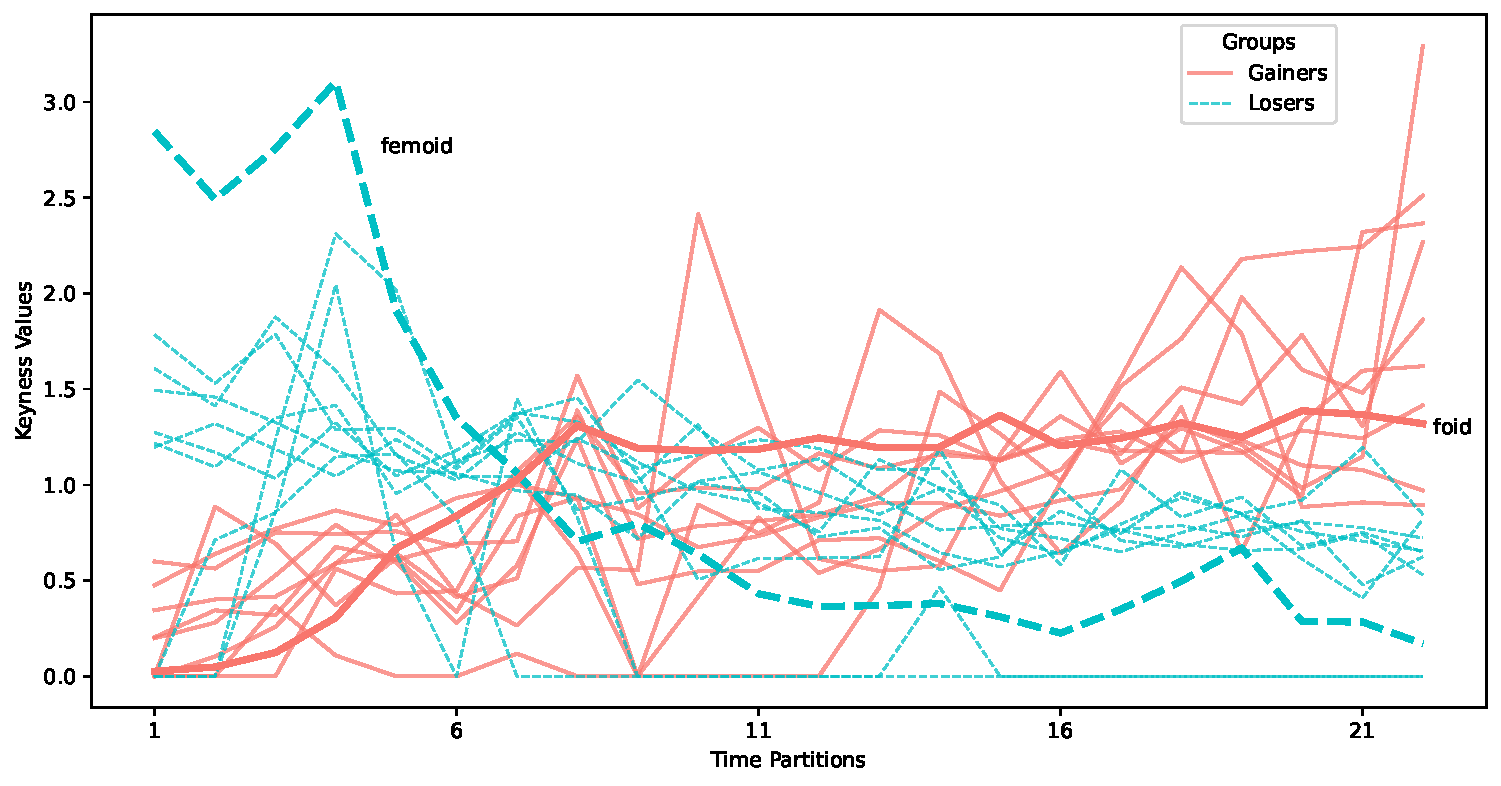
\includegraphics[width=\textwidth]{images-tables/keyness_chart_incelsis.pdf}
    \caption{\enforum}
  \end{subfigure}
  \begin{subfigure}[b]{\textwidth}
    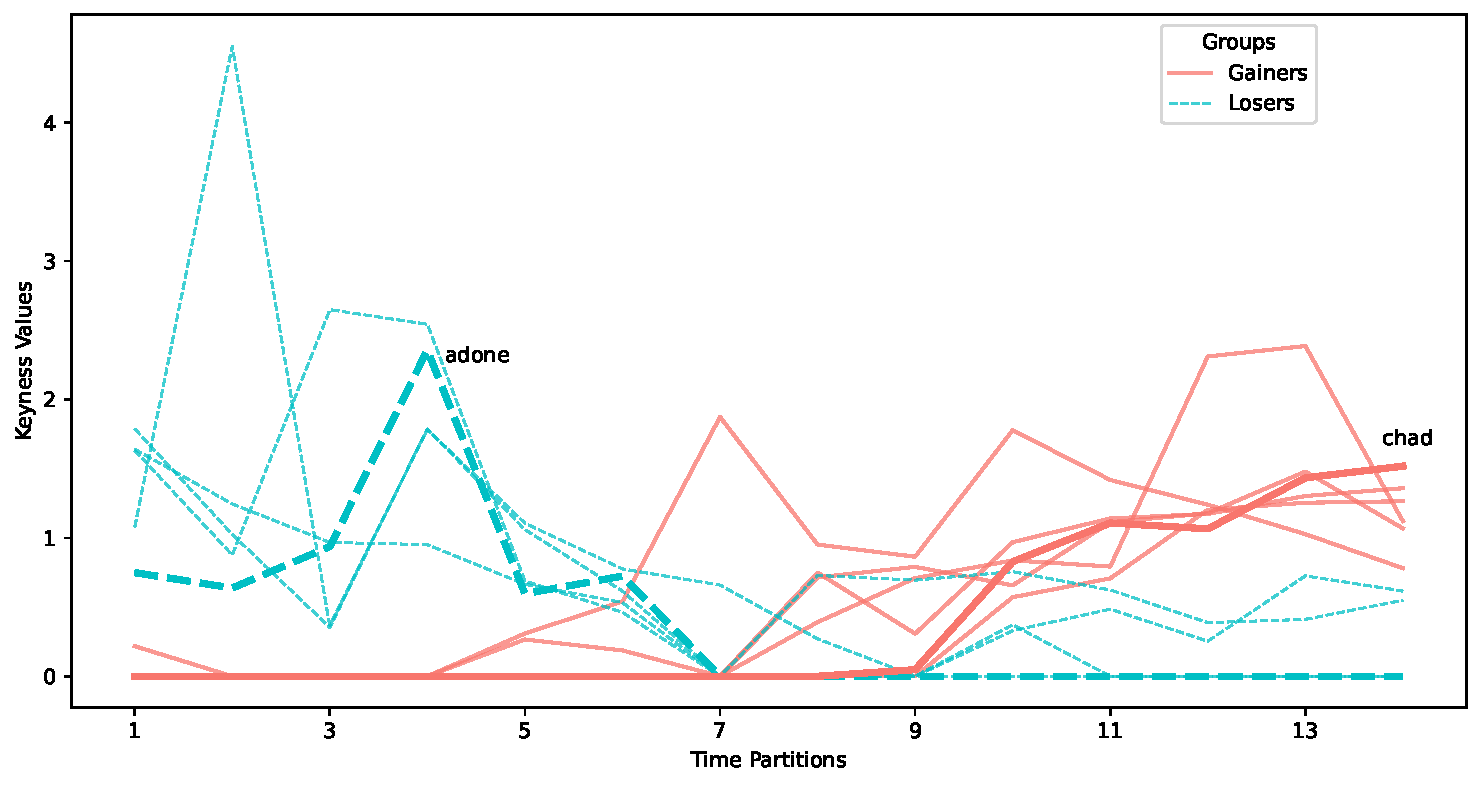
\includegraphics[width=\textwidth]{images-tables/keyness_chart_fdb.pdf}
    \caption{\itforum}
  \end{subfigure}
  \caption[Keyness graph for \enforum\, and \itforum.]{Keyness over time for the characteristic incel terms extracted from the (a) \enforum\, and (b) \itforum\, forums. Red lines represent the terms that gained keyness over time, while blue lines represent the terms that lost keyness over time.}
  \label{fig:keyness-over-time}
\end{figure*}

\begin{table}[t]
  \caption{Keyness normalized slopes for \enforum\, and \itforum.}
  \footnotesize
    \centering
    \begin{tabular}{c|lc|lc}
      \hline
      \multirow{2}{*}[0pt]{\rotatebox[origin=c]{0}{\bf Forum}} & \multicolumn{2}{c|}{\bf Gainers} & \multicolumn{2}{c}{\bf Losers} \\
      \cline{2-5}
       & \bf Term &\bf  Slope &\bf  Term &\bf  Slope \\
      \hline
      \multirow{11}{*}[0pt]{\rotatebox[origin=c]{90}{\enforum}} & shitskin    & 0.093           & racepill    & -0.019           \\
      & deathnic    & 0.081           & stacie      & -0.022           \\
      &cumskin     & 0.079           & jb          & -0.027           \\
      &noodlewhore & 0.077           & chadlite    & -0.029           \\
      &slav        & 0.068           & whitecels   & -0.032           \\
      &foid        & 0.058           & cunt        & -0.036           \\
      &curryland   & 0.051           & slut        & -0.046           \\
      &aryan       & 0.048           & deathnik    & -0.047           \\
      &ricecel     & 0.047           & roastie     & -0.051           \\
      &whore       & 0.025           & femoid      & -0.124           \\
      \cline{2-5}
      &\bf Mean       &\bf 0.063  &\bf Mean       &\bf -0.043      \\
      \hline
      \multirow{6}{*}[8pt]{\rotatebox[origin=c]{90}{\begin{minipage}{2cm}\textit{Il forum}\\ \textit{dei brutti}\end{minipage}}}
      &zerbini & 0.104 & reietto & -0.142 \\
      &normie & 0.121 & strafigo & -0.122 \\
      &bv & 0.125 & figaccione & -0.122 \\
      &chad & 0.126 & attraente & -0.113 \\
      &subumano & 0.158 & adone & -0.103 \\
      \cline{2-5}
      &\bf Mean &\bf 0.127 &\bf Mean &\bf -0.120 \\ \hline
    \end{tabular}
  \label{tab:keyness}
\end{table}

Table~\ref{tab:keyness} reports the normalized slopes of the terms obtained from the two forums. In both cases, the mean normalized slopes of the two data series, compared side by side, quantitatively display a clear trend according to which certain terms gain popularity over time, while others become less popular. With regard to \enforum, the difference between the mean normalized slopes is 0.106, while for \itforum\, the difference is even larger, 0.247, which points at an even faster lexical evolution. In both cases, the shift in lexicon needs to be taken into account in order to have a clear picture of the language adopted by each speech community. For terms such as ``foid'', ``femoid'', and ``roastie'', the observed trends also confirm the time-series data discussed in \newcite{gothard2020ExploringIncelLanguage}, which show certain terms increasing and decreasing in use over the total messages posted in incel subreddits.

With relation to \enforum, as already anticipated through Figure~\ref{fig:keyness-over-time}, although terms like ``foid'' and ``femoid'' have the same meaning (both are used to dehumanize women by associating them to insentient androids\footnote{\url{https://incels.wiki/w/Femoid}}), the shorter form has become more popular, while the use of the full form has decreased. This is probably due to the fact that, given the high frequency with which the term is used in the forum, users tend to use the abbreviated version to save time and effort. This might seem like a minor detail, but the sheer amount of misogyny that is expressed in the forum through this term alone makes it important to point out a shift in its use.

As regards \itforum, we can observe that the way users refer to men changes in a rather clear way. On one hand, positive words that are commonly used in general language, such as ``strafigo'' and ``figaccione'' (both meaning ``extremely handsome''), are substituted by specialized terms that are more specific to the forum's speech community, e.g., ``chad''.\footnote{\url{https://incels.wiki/w/Chad}} On the other hand, we can see the same phenomenon for negative words, where ``reietto'' (``outcast'') loses popularity, leaving space to terms with more specialized uses, such as ``bv'', meaning ``brutto vero'' (lit. ``truly ugly''), and ``subumano'', meaning ``subhuman''. The first is an acronym, which makes its meaning opaque to outsiders, while the second is a term with a much stronger and denigrating connotation.

% This trend is also confirmed statistically. For both forums, we first take the normalized average slopes for each term and then we test if the difference between gainers and losers of keyness is statistically significant. For the \enforum\, forum, since the data series of the losers is not normally distributed, we use the Mann-Whitney U test \cite{mann1947test}. For \itforum, since both data series are normally distributed, we use a two-sample t-test \cite{snedecor1989statistical}. In both cases, the p-values are well below 0.001, as shown in Table~\ref{tab:statistical-tests-diachronic-study}, showing the results are statistically significant. This means that the change in the usage of the terms is not random, but rather due to a concrete variation in the way specific lexicon is used by the two speech communities.

% \begin{table}[t]
%   \centering
%   \caption[Keyness statistical tests.]{Results of the Mann-Whitney U test and the t-test for the normalized slopes of the keyness of the terms gaining and losing popularity over time, for \enforum\, and \itforum, respectively.}
%   \label{tab:statistical-tests-diachronic-study}
%   \begin{tabular}{l|c|c|c}
%     \hline
%   \bf Forum                    &\bf  Test       &\bf  Stat Value  &\bf  \textit{p}-Value        \\
%   \hline
%   \enforum\,           & Mann-Whitney U & 100             & 0.0002             \\
%   \itforum\, & t-test         & -22.7566        & 1.4736 x $10^{-8}$ \\
%   \hline
%   \end{tabular}
%   \end{table}

Based on the conducted qualitative and quantitative analyses, the same conclusions can be drawn for both forums: the presented terms are arguably characteristic of the incel language used within the two platforms and the change in their usage over time is non-negligible. This implies that language models could become progressively worse at predicting over these domains, were their training resources not be periodically updated. Models rely on training material to learn language, and if the material is outdated, their understanding of the discourse currently produced by a specific speech community could become suboptimal. This is especially important considering the fact that, especially in the case of \enforum, the presented racist and misogynous terms are novel and carry most of the discriminatory meaning through neologisms.

Consequently, it seems desirable, if not necessary, to periodically update corpora to have accurate terminological representations. In some cases, it would arguably make sense to even rebuild resources from scratch, were they too outdated. In our case, given the observed changes in keyness, we estimate that the hereby analyzed time frame could be taken as a reference for how long resources can be considered up-to-date. However, with the aim of obtaining an objective figure, further research could be conducted to quantify how often resources should be updated to keep up with the evolution of the language used in the spaces scrutinized through this study.

The necessity to build such material is also supported by the fact that resources on the topic of incels are rare and limited, and their applicability is often compromised because the linguistic domain of the source data only partially aligns with the one under investigation \cite{pelzer-2021-toxic-language-incel-communities}. An additional cause for such incompatibility of resources can be found in the annotation scheme, which can be inapplicable to the supervised task being approached \cite{zhou-2022-automated-hs-detection}. However, the necessity to build new resources does not mean they will be obsolete soon after being employed, as the time frames we have analyzed in this chapter span various years of forum activity.

% \clearpage

% \section{Complete Results}
% \label{app:complete-results}

%   \begin{strip}
%   \centering
%   % \footnotesize
%   \captionof{table}{Performance on the hate speech identification task of the adopted models when fine-tuning them on all combinations of the adopted datasets in English and Italian (top) and only Italian (bottom), for the epoch (e) of maximum validation F$_1$-measure.}
%   \label{tab:hate-speech-all-models-all-ids-appendix}

% \begin{tabular}{l|c@{\hspace{1mm}}|c@{\hspace{1mm}}c@{\hspace{1mm}}c@{\hspace{1mm}}|c@{\hspace{1mm}}|ccc|ccc}
% \multicolumn{1}{c|}{} & \multicolumn{1}{c|}{\bf EN} & \multicolumn{3}{c|}{\bf IT} & \bf (e) & \multicolumn{3}{c|}{\bf \begin{minipage}{3cm}\begin{center}Val. (\dsENclassificationdev)\end{center}\end{minipage}} & \multicolumn{3}{c}{\bf \begin{minipage}{3cm}\begin{center}Test (\dsITclassification)\end{center}\end{minipage}}\\
%  & \rotatebox{90}{Incels.is} & \rotatebox{90}{\hsdfb} & \rotatebox{90}{\hsdtw} & \rotatebox{90}{\ami} &
%  & \bf F$_1$& \bf Rec & \bf Prec & \bf F$_1$& \bf Rec & \bf Prec \\
%     \hline
%         \multirow{7}{*}[0pt]{\rotatebox[origin=c]{90}{\begin{minipage}{1.5cm}mBERT\end{minipage}}} 
%     &  \bs &  \bs  &      &      &      3 &      0.841$\pm$0.004 &     0.852 &       0.832 &       0.688$\pm$0.006 &      0.921 &       0.549 \\ % 34
%     &  \bs &       &  \bs &      &      3 &      0.846$\pm$0.002 &     0.866 &       0.827 &       0.529$\pm$0.041 &      0.482 &       0.588 \\ % 35
%     &  \bs &       &      &  \bs &      5 &      0.844$\pm$0.007 &     0.849 &       0.838 &       0.634$\pm$0.023 &      0.587 &       0.692 \\ % 36
%     &  \bs &  \bs  &  \bs &      &      4 &      0.844$\pm$0.006 &     0.844 &       0.844 &       0.616$\pm$0.028 &      0.675 &       0.568 \\ % 37
%     &  \bs &  \bs  &      &  \bs &      5 &      0.842$\pm$0.004 &     0.844 &       0.840 &       0.676$\pm$0.012 &      0.801 &       0.585 \\ % 38
%     &  \bs &       &  \bs &  \bs &      4 &      0.847$\pm$0.008 &     0.841 &       0.853 &       0.570$\pm$0.048 &      0.535 &       0.620 \\ % 39
%     &  \bs &  \bs  &  \bs &  \bs &      5 &      0.837$\pm$0.008 &     0.829 &       0.845 &       0.613$\pm$0.019 &      0.639 &       0.590 \\ % 40
%     \hline
%         \multirow{7}{*}[0pt]{\rotatebox[origin=c]{90}{\begin{minipage}{2.2cm}Incel mBERT\end{minipage}}} 
%     &  \bs &  \bs  &      &      &      5 &      0.859$\pm$0.010 &     0.853 &       0.864 &       0.708$\pm$0.007 &      0.889 &       0.588 \\ % 34
%     &  \bs &       &  \bs &      &      2 &      0.861$\pm$0.015 &     0.866 &       0.856 &       0.615$\pm$0.025 &      0.558 &       0.690 \\ % 35
%     &  \bs &       &      &  \bs &      4 &      0.853$\pm$0.009 &     0.863 &       0.844 &       0.722$\pm$0.028 &      0.704 &       0.746 \\ % 36
%     &  \bs &  \bs  &  \bs &      &      5 &      0.857$\pm$0.007 &     0.855 &       0.859 &       0.679$\pm$0.014 &      0.731 &       0.635 \\ % 37
%     &  \bs &  \bs  &      &  \bs &      4 &      0.856$\pm$0.009 &     0.857 &       0.856 &       0.689$\pm$0.011 &      0.707 &       0.673 \\ % 38
%     &  \bs &       &  \bs &  \bs &      5 &      0.850$\pm$0.007 &     0.839 &       0.860 &       0.644$\pm$0.010 &      0.580 &       0.725 \\ % 39
%     &  \bs &  \bs  &  \bs &  \bs &      5 &      0.869$\pm$0.003 &     0.878 &       0.861 &       0.700$\pm$0.013 &      0.702 &       0.698 \\ % 40
%     \hline
%     % \multicolumn{1}{c}{} \\
%     \multicolumn{1}{c}{} & \multicolumn{1}{c}{} & \multicolumn{1}{c}{} & \multicolumn{1}{c}{} & \multicolumn{1}{c}{} & \multicolumn{3}{c}{\bf \begin{minipage}{3cm}\begin{center}Val. (Italian)\end{center}\end{minipage}} & \multicolumn{3}{c}{\bf \begin{minipage}{3cm}\begin{center}Test (\dsITclassification)\end{center}\end{minipage}}\\
%     \hline
%     \multirow{7}{*}[0pt]{\rotatebox[origin=c]{90}{\begin{minipage}{1.7cm}\umbert\end{minipage}}} 
%     &      &  \bs  &      &      &      5 &      0.855$\pm$0.003 &     0.868 &       0.843 &       0.696$\pm$0.010 &      0.879 &       0.576 \\ % 27
%     &      &       &  \bs &      &      4 &      0.754$\pm$0.004 &     0.800 &       0.713 &       0.432$\pm$0.060 &      0.319 &       0.685 \\ % 28
%     &      &       &      &  \bs &      4 &      0.914$\pm$0.004 &     0.931 &       0.899 &       0.569$\pm$0.031 &      0.520 &       0.631 \\ % 29
%     &      &  \bs  &  \bs &      &      4 &      0.788$\pm$0.006 &     0.824 &       0.755 &       0.666$\pm$0.024 &      0.758 &       0.595 \\ % 30
%     &      &  \bs  &      &  \bs &      5 &      0.883$\pm$0.004 &     0.900 &       0.867 &       0.697$\pm$0.019 &      0.747 &       0.653 \\ % 31
%     &      &       &  \bs &  \bs &      5 &      0.828$\pm$0.003 &     0.844 &       0.814 &       0.596$\pm$0.017 &      0.526 &       0.688 \\ % 32
%     &      &  \bs  &  \bs &  \bs &      5 &      0.822$\pm$0.003 &     0.836 &       0.808 &       0.680$\pm$0.016 &      0.692 &       0.671 \\ % 33
%     \hline
%     \multirow{7}{*}[0pt]{\rotatebox[origin=c]{90}{\begin{minipage}{2.6cm} \iumbert\end{minipage}}} 
%     &      &  \bs  &      &      &      5 &      0.867$\pm$0.006 &     0.887 &       0.848 &       0.705$\pm$0.009 &      0.870 &       0.593 \\ % 27
%     &      &       &  \bs &      &      4 &      0.756$\pm$0.002 &     0.810 &       0.708 &       0.403$\pm$0.024 &      0.285 &       0.692 \\ % 28
%     &      &       &      &  \bs &      4 &      0.918$\pm$0.001 &     0.946 &       0.891 &       0.652$\pm$0.031 &      0.608 &       0.705 \\ % 29
%     &      &  \bs  &  \bs &      &      4 &      0.790$\pm$0.003 &     0.831 &       0.754 &       0.660$\pm$0.014 &      0.696 &       0.627 \\ % 30
%     &      &  \bs  &      &  \bs &      5 &      0.886$\pm$0.002 &     0.901 &       0.872 &       0.704$\pm$0.005 &      0.732 &       0.678 \\ % 31
%     &      &       &  \bs &  \bs &      2 &      0.831$\pm$0.003 &     0.866 &       0.799 &       0.648$\pm$0.011 &      0.544 &       0.802 \\ % 32
%     &      &  \bs  &  \bs &  \bs &      5 &      0.828$\pm$0.003 &     0.853 &       0.804 &       0.699$\pm$0.029 &      0.718 &       0.682 \\ % 33
%     \hline
%     \multirow{7}{*}[0pt]{\rotatebox[origin=c]{90}{\begin{minipage}{1.7cm}\albert\end{minipage}}} 
%     &      &  \bs  &      &      &      4 &      0.850$\pm$0.003 &     0.899 &       0.807 &       0.683$\pm$0.006 &      0.941 &       0.537 \\ % 27
%     &      &       &  \bs &      &      1 &      0.752$\pm$0.006 &     0.817 &       0.698 &       0.520$\pm$0.089 &      0.426 &       0.716 \\ % 28
%     &      &       &      &  \bs &      2 &      0.907$\pm$0.004 &     0.952 &       0.866 &       0.528$\pm$0.022 &      0.517 &       0.542 \\ % 29
%     &      &  \bs  &  \bs &      &      2 &      0.775$\pm$0.003 &     0.803 &       0.750 &       0.695$\pm$0.007 &      0.786 &       0.623 \\ % 30
%     &      &  \bs  &      &  \bs &      3 &      0.879$\pm$0.003 &     0.918 &       0.843 &       0.705$\pm$0.011 &      0.803 &       0.629 \\ % 31
%     &      &       &  \bs &  \bs &      3 &      0.820$\pm$0.001 &     0.888 &       0.762 &       0.652$\pm$0.018 &      0.645 &       0.660 \\ % 32
%     &      &  \bs  &  \bs &  \bs &      2 &      0.808$\pm$0.011 &     0.872 &       0.753 &       0.684$\pm$0.015 &      0.821 &       0.587 \\ % 33
%     \hline
%     \multirow{7}{*}[0pt]{\rotatebox[origin=c]{90}{\begin{minipage}{2.6cm} \ialbert\end{minipage}}} 
%     &      &  \bs  &      &      &      5 &      0.847$\pm$0.005 &     0.863 &       0.831 &       0.707$\pm$0.007 &      0.791 &       0.639 \\ % 27
%     &      &       &  \bs &      &      1 &      0.748$\pm$0.002 &     0.785 &       0.715 &       0.506$\pm$0.035 &      0.370 &       0.805 \\ % 28
%     &      &       &      &  \bs &      5 &      0.912$\pm$0.003 &     0.930 &       0.895 &       0.617$\pm$0.018 &      0.562 &       0.685 \\ % 29
%     &      &  \bs  &  \bs &      &      2 &      0.771$\pm$0.004 &     0.791 &       0.752 &       0.673$\pm$0.016 &      0.721 &       0.632 \\ % 30
%     &      &  \bs  &      &  \bs &      5 &      0.873$\pm$0.003 &     0.888 &       0.858 &       0.668$\pm$0.014 &      0.663 &       0.674 \\ % 31
%     &      &       &  \bs &  \bs &      1 &      0.818$\pm$0.004 &     0.864 &       0.776 &       0.656$\pm$0.007 &      0.593 &       0.736 \\ % 32
%     &      &  \bs  &  \bs &  \bs &      4 &      0.800$\pm$0.009 &     0.828 &       0.773 &       0.688$\pm$0.017 &      0.747 &       0.639 \\ % 33
%     \hline
% \end{tabular}
% \end{strip}

% \begin{tabular}{lrrrrrrrrr}
%                Model &  (e)   &   Val F1          &  Val Rec &  Val Prec &    Test F1         &  Test Rec &  Test Prec \\ % ID
%              \albert\, &      4 &   0.850$\pm$0.003 &    0.899 &     0.807 &    0.683$\pm$0.006 &     0.941 &      0.537 \\ % 27
%              \albert\, &      1 &   0.752$\pm$0.006 &    0.817 &     0.698 &    0.520$\pm$0.089 &     0.426 &      0.716 \\ % 28
%              \albert\, &      2 &   0.907$\pm$0.004 &    0.952 &     0.866 &    0.528$\pm$0.022 &     0.517 &      0.542 \\ % 29
%              \albert\, &      2 &   0.775$\pm$0.003 &    0.803 &     0.750 &    0.695$\pm$0.007 &     0.786 &      0.623 \\ % 30
%              \albert\, &      3 &   0.879$\pm$0.003 &    0.918 &     0.843 &    0.705$\pm$0.011 &     0.803 &      0.629 \\ % 31
%              \albert\, &      3 &   0.821$\pm$0.001 &    0.886 &     0.764 &    0.646$\pm$0.019 &     0.630 &      0.665 \\ % 32
%   Incel \albert\, 627k &      5 &   0.847$\pm$0.005 &    0.863 &     0.831 &    0.707$\pm$0.007 &     0.791 &      0.639 \\ % 27
%   Incel \albert\, 627k &      1 &   0.748$\pm$0.002 &    0.785 &     0.715 &    0.506$\pm$0.035 &     0.370 &      0.805 \\ % 28
%   Incel \albert\, 627k &      5 &   0.912$\pm$0.003 &    0.930 &     0.895 &    0.617$\pm$0.018 &     0.562 &      0.685 \\ % 29
%   Incel \albert\, 627k &      2 &   0.771$\pm$0.004 &    0.791 &     0.752 &    0.673$\pm$0.016 &     0.721 &      0.632 \\ % 30
%   Incel \albert\, 627k &      5 &   0.873$\pm$0.003 &    0.888 &     0.858 &    0.668$\pm$0.014 &     0.663 &      0.674 \\ % 31
%   Incel Umberto 627k &      5 &   0.867$\pm$0.006 &    0.887 &     0.848 &    0.705$\pm$0.009 &     0.870 &      0.593 \\ % 27
%   Incel Umberto 627k &      4 &   0.756$\pm$0.002 &    0.810 &     0.708 &    0.403$\pm$0.024 &     0.285 &      0.692 \\ % 28
%   Incel Umberto 627k &      4 &   0.918$\pm$0.001 &    0.946 &     0.891 &    0.652$\pm$0.031 &     0.608 &      0.705 \\ % 29
%   Incel Umberto 627k &      4 &   0.790$\pm$0.003 &    0.831 &     0.754 &    0.660$\pm$0.014 &     0.696 &      0.627 \\ % 30
%   Incel Umberto 627k &      5 &   0.886$\pm$0.002 &    0.901 &     0.872 &    0.704$\pm$0.005 &     0.732 &      0.678 \\ % 31
%       Incel mBERT 1M &      5 &   0.859$\pm$0.010 &    0.853 &     0.864 &    0.708$\pm$0.007 &     0.889 &      0.588 \\ % 34
%       Incel mBERT 1M &      2 &   0.861$\pm$0.015 &    0.866 &     0.856 &    0.615$\pm$0.025 &     0.558 &      0.690 \\ % 35
%       Incel mBERT 1M &      4 &   0.853$\pm$0.009 &    0.863 &     0.844 &    0.722$\pm$0.028 &     0.704 &      0.746 \\ % 36
%       Incel mBERT 1M &      5 &   0.857$\pm$0.007 &    0.855 &     0.859 &    0.679$\pm$0.014 &     0.731 &      0.635 \\ % 37
%       Incel mBERT 1M &      4 &   0.856$\pm$0.009 &    0.857 &     0.856 &    0.689$\pm$0.011 &     0.707 &      0.673 \\ % 38
%       Incel mBERT 1M &      5 &   0.850$\pm$0.007 &    0.839 &     0.860 &    0.644$\pm$0.010 &     0.580 &      0.725 \\ % 39
%       Incel mBERT 1M &      5 &   0.869$\pm$0.003 &    0.878 &     0.861 &    0.700$\pm$0.013 &     0.702 &      0.698 \\ % 40
%              Umberto &      5 &   0.855$\pm$0.003 &    0.868 &     0.843 &    0.696$\pm$0.010 &     0.879 &      0.576 \\ % 27
%              Umberto &      4 &   0.754$\pm$0.004 &    0.800 &     0.713 &    0.432$\pm$0.060 &     0.319 &      0.685 \\ % 28
%              Umberto &      4 &   0.914$\pm$0.004 &    0.931 &     0.899 &    0.569$\pm$0.031 &     0.520 &      0.631 \\ % 29
%              Umberto &      4 &   0.788$\pm$0.006 &    0.824 &     0.755 &    0.666$\pm$0.024 &     0.758 &      0.595 \\ % 30
%              Umberto &      5 &   0.883$\pm$0.004 &    0.900 &     0.867 &    0.697$\pm$0.019 &     0.747 &      0.653 \\ % 31
%           mBERT base &      3 &   0.841$\pm$0.004 &    0.852 &     0.832 &    0.688$\pm$0.006 &     0.921 &      0.549 \\ % 34
%           mBERT base &      3 &   0.846$\pm$0.002 &    0.866 &     0.827 &    0.529$\pm$0.041 &     0.482 &      0.588 \\ % 35
%           mBERT base &      5 &   0.844$\pm$0.007 &    0.849 &     0.838 &    0.634$\pm$0.023 &     0.587 &      0.692 \\ % 36
%           mBERT base &      4 &   0.844$\pm$0.006 &    0.844 &     0.844 &    0.616$\pm$0.028 &     0.675 &      0.568 \\ % 37
%           mBERT base &      5 &   0.842$\pm$0.004 &    0.844 &     0.840 &    0.676$\pm$0.012 &     0.801 &      0.585 \\ % 38
%           mBERT base &      4 &   0.847$\pm$0.008 &    0.841 &     0.853 &    0.570$\pm$0.048 &     0.535 &      0.620 \\ % 39
%           mBERT base &      5 &   0.837$\pm$0.008 &    0.829 &     0.845 &    0.613$\pm$0.019 &     0.639 &      0.590 \\ % 40
%   \end{tabular}

\end{document}
